\documentclass{article}

\usepackage[frenchb]{babel}
\usepackage{amsfonts}
\usepackage{amsmath}
\usepackage{amssymb}
%\usepackage[T1]{fontenc}
\usepackage[utf8]{inputenc}
\usepackage{amsthm}
\usepackage{graphicx}
\usepackage{tikz}
\usepackage{tikz-cd}
\usepackage{hyperref}
\usepackage{amssymb}
\usepackage{geometry}

\hypersetup{                    % parametrage des hyperliens
    colorlinks=true,                % colorise les liens
    breaklinks=true,                % permet les retours à la ligne pour les liens trop longs
    urlcolor= blue,                 % couleur des hyperliens
    linkcolor= blue,                % couleur des liens internes aux documents (index, figures, tableaux, equations,...)
    citecolor= cyan               % couleur des liens vers les references bibliographiques
    }

\theoremstyle{definition}
\newtheorem{definition}{Definition}
\newtheorem{thm}{Theorem}
\newtheorem{ex}{Exercice}
\newtheorem{lem}{Lemma}
\newtheorem*{dem}{Proof}
\newtheorem{prop}{Proposition}
\newtheorem{cor}{Corollary}
\newtheorem{conj}{Conjecture}
\newtheorem{Res}{Result}
\newtheorem{Expl}{Example}
\newtheorem{rk}{Remark}

\newcommand{\N}{\mathbb N}
\newcommand{\Z}{\mathbb Z}
\newcommand{\R}{\mathbb R}
\newcommand{\C}{\mathbb C}
\newcommand{\Hil}{\mathcal H}
\newcommand{\Mn}{\mathcal M _n (\mathbb C)}
\newcommand{\K}{\mathbb K}
\newcommand{\B}{\mathbb B}
\newcommand{\Cat}{\mathbb B / \mathbb K}
\newcommand{\G}{\mathcal G }

\setlength\parindent{0pt}



\title{Introduction à la K-théorie des $C^*$-algèbres}
\date{}
\author{ Clément Dell'Aiera}




\begin{document}
\maketitle
\begin{figure}[h]\centering
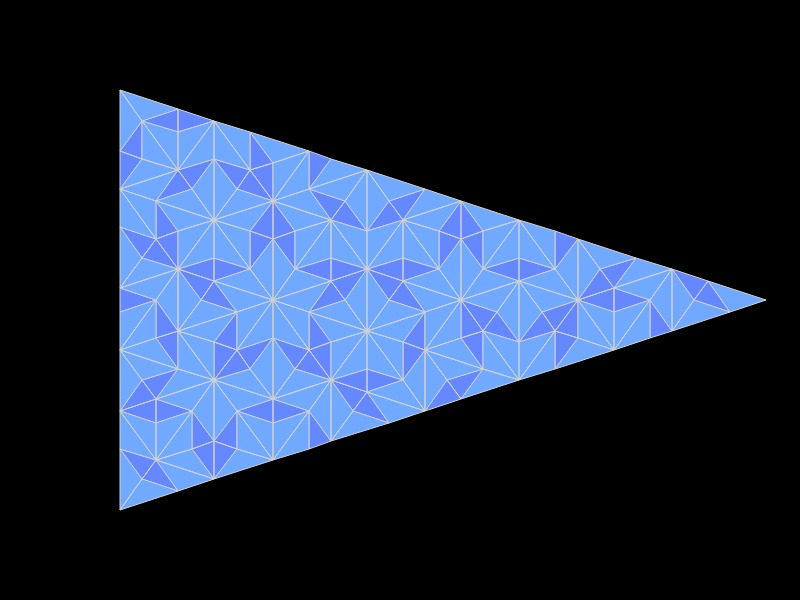
\includegraphics[scale=0.4]{Penrose.png}
\caption{Pavage de Penrose généré avec http://www.spacegoo.com/penrose/}
\label{fig:Penrose}
\end{figure}

\newpage
\tableofcontents

\newpage

\section{Introduction}
\subsection{Notations}

Pour une $C^*$-algèbre $A$ non nécessairement unitale, on note $A^+$ la $C^*$-algèbre unitale qui la contient en tant qu'idéal bilatère, définie par :

\[\begin{array}{c}A^+=\{(a,\lambda)\in A\times \C \} \\ (a,\lambda)(b,\mu)=(ab+\lambda b +\mu a,\lambda\mu) \\ (a,\lambda)^*=(a^*,\overline\lambda)\end{array}\]
et munie de la norme d'opérateur
\[||(a,\lambda)||=\sup \{||ax+\lambda x|| : x\in A , ||x||=1\}.\]
 On a alors une suite exacte :
\[\begin{tikzcd}[column sep = small] 0 \arrow{r} &  A \arrow{r} & A^+ \arrow{r}{\pi_\C} & \C \arrow{r} & 0 \end{tikzcd}.\]

On rappelle que pour tout semi-groupe abélien $S$, il existe un groupe $G_S$, appelé groupe de Grothendieck de $S$, et un morphisme de semi-groupe $\mu : S\rightarrow G_S$ tels que, pour tout groupe $G$ et tout morphisme de semi-groupe $\alpha : S\rightarrow G$, il existe un unique morphisme de groupe $\tilde \alpha : G_S \rightarrow G$ vérifiant $\alpha = \mu \circ \tilde\alpha$. 

\[\begin{tikzcd} S \arrow{r}{\alpha} \arrow[dotted]{d}{\exists !\tilde\alpha}& G \\
	G_S \arrow{ur}{\mu} & \end{tikzcd}\]
 Voici une construction explicite de $G_S$. On considère $S\times S$ que l'on muni de la relation d'équivalence 
\[(x,y)\sim (x',y') \quad \text{ssi} \quad \exists r \in S/ x+y'+r=x'+y+r.\]
Alors $S\times S/ \sim$ est un groupe où la classe de $(x,x)$ est constante pour tout $x\in S$, et donne le neutre du groupe. L'inverse de la classe de $(x,y)$ est quant à lui donné par la classe de $(y,x)$. On écrira $[x]-[y]$ pour la classe de $(x,y)$.\\

Enfin, une remarque sur les limites inductives de $C^*$-algèbres. Par système inductif, on entend une famille de morphismes $\{\phi_{ij}:A_j\rightarrow A_i\}_{i>j}$, où $i$ et $j$ sont éléments d'un ensemble partiellement ordonné, vérifiant la condition de cohérence :
\[\phi_{ij}\circ\phi_{jk}=\phi_{ik}\quad \text{si }\ i>j>k.\]
Il existe alors un objet universel $A_\infty$, appelé la limite inductive algébrique du système $\{A_i; \phi_{ij}\}$, et des morphismes canoniques $\phi_i : A_i \rightarrow A_\infty$ qui rendent le diagramme suivant commutatif :
\[\begin{tikzcd} A_i \arrow{r}{\phi_i} & A_\infty \\
			A_j \arrow{ur}{\phi_j}\arrow{u}{\phi_{ij}} & 
\end{tikzcd}\]
et tel que $A_\infty = \cup \phi_j(A_j)$. Cet objet est universel au sens où, pour tout autre $A'_\infty$ et morphismes $\phi_i' : A_i\rightarrow A'_\infty$ qui font commuter le précédent diagramme, alors il existe un unique morphisme $A_\infty \rightarrow A'_\infty$ tel que le diagramme :
\[\begin{tikzcd}A_i \arrow{r}{\phi_i}\arrow{dr}{\phi'_i}& A_\infty\arrow[dotted]{d} \\
		    A_j \arrow{u}{\phi_{ij}}\arrow{ur}{\phi_j}\arrow{r}{\phi'_j}& A'_\infty
\end{tikzcd}\] 
commute. De plus, si chaque $\phi'_j$ est injectif, la flèche en pointillés l'est aussi. Et elle est surjective si $A_\infty= \cup \phi'_j A_j$. \\

Si $x=\phi_j(a_j)$,
\[\alpha(x):=\sup_i\{||\phi_{ij}(a_j)||\}\]
définit une semi-$C*$-norme sur $A_\infty$. On peut alors quotienter par l'idéal des éléments qui annulent $\alpha$, puis compléter par rapport à la norme obtenue sur le quotient. On étend ainsi la limite inductive à la catégorie des $C^*$-algèbre. Dans la suite de ce rapport, lorsque l'on parlera de limite inductive, cela désignera par défaut cette construction.
 
\subsection{Rappels sur les produits tensoriels de $C^*$-algèbres}

Cette section présente les résultats qui seront utilisés sur les produits tensoriels de $C^*$-algèbres. Toutes les preuves des affirmations non justifiées peuvent être trouvées dans le livre de Murphy ~\cite{Murphy} par exemple.\\

On rappelle que le produit tensoriel de $2$ espaces vectoriels $E$ et $F$ est défini comme l'unique (à isomorphisme près) espace vectoriel $E\otimes F$ muni d'une application bilinéaire $\pi : E\times F \rightarrow E\otimes F$ tel que, pour tout espace vectoriel $W$ et toute application bilinéaire $\phi : E \times F \rightarrow W $, il existe une unique application linéaire $\varphi :E\otimes F \rightarrow W$ telle que $\phi = \varphi\circ \pi$. On note $\pi(x,y)=x\otimes y$. Ce sont ces éléments, appelés tenseurs élémentaires, qui engendrent $E\otimes F$ comme espace vectoriel.\\ 

Le lemme suivant donne l'unicité à isomorphisme près :

\begin{lem}
Soient $E$ et $F$ deux espaces vectoriels sur un corps $K$. S'il existe deux $K$-espaces vectoriels $V_1$ et $V_2$ munis d'applications bilinéaires $\pi_j : E\times F \rightarrow V_j$ telles que, pour tout espace vectoriel $W$, toute application bilinéaire $E\times F \rightarrow W$,  se factorise uniquement via $\pi_1$ et $\pi_2$, alors $V_1$ et $V_2$ sont isomorphes en tant que $K$-espaces vectoriels.
\end{lem}


\[\begin{tikzcd}
V_1 \arrow{dr}& \arrow{l}{\pi_1}	E\times F \arrow{d}\arrow{r}{\pi_2}	& \arrow{dl}V_2 \\
			 & 		W		&	\\
\end{tikzcd}\]

\begin{dem}
En appliquant la propriété d'unique factorisation aux deux applications $\pi_j$ elles-mêmes, il existe deux uniques applications linéaires $\phi_1 : V_2\rightarrow V_1$ et $\phi_2 : V_1\rightarrow V_2$ telles que :
\[\begin{array}{c}\pi_1=\phi_1\circ \pi_2 \\ \pi_2=\phi_2\circ \pi_1.\end{array}\]

Montrons que ces deux applications sont inverses. Comme :
\[\phi_1\circ \phi_2 \circ \pi_1 = \phi_1\circ \pi_2 =\pi_1 ,\]
$\phi_1\circ \phi_2 = id_{V_1}$ par unicité de la factorisation de $\pi_1$ via $\pi_1$.
Symétriquement, on démontre que : $\phi_2\circ \phi_1 = id_{V_2}$, et le résultat est démontré.\\
\qed
\end{dem}

Le problème qui va se poser, si l'on veut définir des produits tensoriels d'espaces vectoriels topologiques par exemple, est celui de la topologie que l'on veut définir sur celui-ci. Alexandre Grothendieck a étudié ces constructions dans sa thèse, voir le séminaire Bourbaki ~\cite{GrothendieckNuc} pour une présentation. C'est au cours de sa thèse que A. Grothendieck a d'ailleurs introduit la nucléarité, notion clé pour les $C^*$-algèbres. On verra en effet que les $C^*$-algèbres nucléaires sont exactes : le foncteur obtenu en tensorisant par elle-même préserve l'exactitude des complexes de $C^*$-algèbres.\\

Sur les espaces de Hilbert, notre travail est simplifié : il existe un unique produit scalaire sur le produit tensoriel algébrique vérifiant : $\langle x\otimes x', y\otimes y'\rangle=\langle x, y\rangle \langle x',y' \rangle$. La complétion du produit tensoriel algébrique de $H$ et $K$ par rapport à ce produit scalaire est noté $H\hat \otimes K$. Ce résultat peut alors être transféré aux $C^*$-algèbres, grâce à leurs représentations sur des espaces de Hilbert. 

\begin{prop}
Soit $A$ et $B$ deux $C^*$-algèbres et $(H,\varphi)$ et $(K,\psi)$ deux représentations associées. Alors, il existe un unique $*$-homomorphisme $\pi : A\otimes B \rightarrow B(H\hat\otimes K)$ tel que $\pi(a\otimes b)= \varphi(a)\otimes \psi(b)$. De plus, $\pi$ est injectif si $\varphi$ et $\psi$ le sont.
\end{prop} 

On appelle représentation universelle d'une $C^*$-algèbre $A$ la somme directe de toutes les représentations $(H_\tau,\phi_\tau)$, $\tau$ parcourant l'espace des états de $A$, la représentation associée dérivant de la construction GNS. On peut alors définir deux normes sur le produit tensoriel algébrique de $2$ $C^*$-algèbres $A$ et $B$.

\begin{definition}
Soit $A$ et $B$ deux $C^*$-algèbres de représentations universelles $(H_A, \phi_A)$ et $(H_B, \phi_B)$. Soit $\pi$ l'unique $*$-homomorphisme donné par la proposition précédente : $\pi(a\otimes b ) = \phi_A(a)\otimes \phi_B(b)$.
\begin{itemize}
\item Le produit tensoriel spatial $A\otimes_{min} B$ est défini comme la complétion du produit tensoriel algébrique $A\otimes B$ par rapport à la norme 
\[||.||_{min}\left\{\begin{array}{rcl} A\otimes B & \rightarrow & \R_+ \\ c & \mapsto & ||\pi(c)||\end{array}\right.\]
\item Le produit tensoriel maximal $A\otimes_{max} B$ est défini comme la complétion du produit tensoriel algébrique $A\otimes B$ par rapport à la norme 
\[||.||_{max}\left\{\begin{array}{rcl} A\otimes B & \rightarrow & \R_+ \\ c & \mapsto & \max_{p} p(c)\end{array}\right.\]
où $p$ parcourt l'ensemble des semi-$C^*$-normes sur $A\otimes B$.
\end{itemize}
\end{definition}

On se servira de la propriété suivante : pour tout $*$-homomorphismes de $C^*$-algèbres $\varphi : A\rightarrow B$ et $\psi :  A'\rightarrow B'$, il existe un unique $*$-homomorphisme $\pi : A\otimes_{min} A' \rightarrow B\otimes_{min} B'$ tel que 
\[\pi(a\otimes a')=\varphi(a)\otimes \psi (a')\quad , \forall a\in A,a'\in A'.\]
De plus, $\pi $ est injective si $\varphi$ et $\psi$ le sont. On notera $\varphi\otimes_{min}\psi$ à la place de $\pi$ .\\

\begin{definition}
Une $C^*$-algèbre est dite nucléaire s'il n'existe qu'une seule $C^*$-norme sur le produit tensoriel algébrique $A\otimes B$, pour toute $C^*$-algèbre $B$.
\end{definition}

Dans les parties suivantes de ce rapport, lorsque l'on tensorisera par des $C^*$-algèbres nucléaires, on omettra le symbole $min$, et le produit tensoriel topologique sera noté comme  le produit tensoriel algébrique.

\begin{thm}
Soit $B$ une $C^*$-algèbre et
\begin{tikzcd}[column sep = small, row sep = tiny]
0 \arrow{r} & A' \arrow{r}{\varphi} & A \arrow{r}{\psi} & A'' \arrow{r} & 0 \\
\end{tikzcd}
une suite exacte de $C^*$-algèbres. Si le produit tensoriel algébrique $A''\otimes B$ n'admet qu'une seule $C^*$-norme, ce qui arrive lorsque $A''$ ou $B$ est nucléaire, alors la suite 
\[\begin{tikzcd}[column sep = small, row sep = tiny]
0 \arrow{r} & A' \otimes_{min} B\arrow{r}{\tilde\varphi} & A\otimes_{min} B \arrow{r}{\tilde\psi} & A'' \otimes_{min} B\arrow{r} & 0 \\
\end{tikzcd}\]
reste exacte.\\
On a noté $\tilde\varphi=\varphi\otimes_{min} id_B$ et $\tilde\psi = \psi\otimes_{min} id_B$.
\label{Nuclear}
\end{thm}

\begin{dem}
Soit $a''\otimes b \in A''\otimes B$. Par surjectivité, il existe $a\in A$ tel que $\psi(a)=a''$, et donc $\tilde\psi(a\otimes b ) = a''\otimes b$. Les éléments $a''\otimes b$ générant $A''\otimes B$, $\tilde \psi$ est surjective.\\

L'identité de $B$ et $\varphi$ étant des $*$-homomorphismes injectifs, $\tilde\varphi = \varphi \otimes_{min}id_B$ est injectif.\\

Observons que $\text{Im} \ \tilde\varphi =\text{Im}\ \varphi \otimes_{min} B\subset A\otimes_{min} B$ est un idéal.  On vérifie facilement que $\text{Im} \ \tilde\varphi \subset \text{ker}\ \tilde \psi $. Soit donc $R=\text{Im} \ \tilde\varphi$ et $f$ l'application canonique $(A\otimes_{min} B)/ R \rightarrow A''\otimes_{min} B$ obtenue en factorisant $\tilde \psi$. Nous allons construire une application $g : A''\otimes_{min} B \rightarrow (A\otimes_{min} B)/ R $ qui vérifie $g\circ f = id $. Cela montrera que $f$ est injective et donc que $\text{Im} \ \tilde\varphi = \text{ker}\ \tilde \psi $.\\

Soit $a''\in A''$. On choisit $a\in A$ tels que $\psi(a)=a''$ et on définit : 
\[\begin{array}{rcl}
A''\times B & \rightarrow & (A\otimes B) /R \\
a'', b          & \mapsto     & a\otimes b \ (\text{mod} \ R)\\
\end{array}\] 

Cette application ne dépend pas de la préimage de $a''$ choisie : si $\psi(a_1)=\psi(a_2)=a''$, alors $\psi(a_1-a_2)=0$ donc $a_1-a_2=\varphi(a')$ pour un certain $a'\in A'$, d'où $a_1\otimes b -a_2\otimes b = \varphi(a')\otimes b$ et donc $a_1\otimes b = a_2\otimes b \quad \text{mod}\ R$.\\
De plus, la fonction $A''\otimes B\rightarrow \R_+ :  x\mapsto \max (||g(x)||, ||x||_{min})$ est une $C^*$-norme. Par hypothèse, elle est donc égale à $||.||_{min}$, ce qui montre que $g$ est continue.
Etant bilinéaire et continue, cette application se factorise en l'application $g : A''\otimes_{min} B \rightarrow (A\otimes_{min} B) /R$ recherchée. En effet :
\[gf(a\otimes b + R )= g\tilde\psi(a\otimes b)= g(\psi(a)\otimes b)=a\otimes b +R\]
donc $g\circ f = id_{(A\otimes_{min} B)/R}$.

\qed
\end{dem}

Ce théorème sera utile pour la construction de l'extension de Toeplitz. Il sert aussi à la preuve du 

\begin{thm}
Soit
\begin{tikzcd}[column sep = small, row sep = tiny]
0 \arrow{r} & A' \arrow{r}{\varphi} & A \arrow{r}{\psi} & A'' \arrow{r} & 0 \\
\end{tikzcd}
une suite exacte de $C^*$-algèbres. Si $A'$ et $A''$ sont nucléaires, alors $A$ l'est aussi.
\label{NucExtension}
\end{thm}

Les $C^*$-algèbres finies dimensionelles ainsi que les $C^*$-algèbres commutatives sont nucléaires.

\subsection{Applications complètement positives et suites exactes}

Une application bornée $\sigma : A \rightarrow B$ entre deux $C^*$-algèbres unitales est dite complètement positive si $\sigma (1)=1$ et :
\[\sum_{i,j} b_i\sigma(a_i a_j^*) b_j^* \geq 0\]
pour tout entier $n$, tout $a_1$, ...,$a_n$ dans $A$ et $b_1$, ..., $b_n$ dans $B$. \\
Le résultat suivant caractérise les applications complètement positives.

\begin{thm}[Stinespring]
Soit $A$ une $C^*$-algèbre unitale. Une application unitale $\sigma : A \rightarrow B(H)$ est complètement positive ssi il existe :
\begin{itemize}
\item une isométrie $V : H \rightarrow H_1$  
\item une représentation non-dégénérée $\rho : A \rightarrow B(H_1)$
\end{itemize} 
telles que $\sigma(a)=V^*\rho(a)V$ pour tout $a\in A$.
\end{thm}

Ce résultat permet de montrer que si $\sigma : A \rightarrow A'$ est une application complètement positive, alors l'application $\sigma \otimes 1$, définie sur le produit tensoriel algébrique de manière évidente, s'étend en une application complètement positive $\sigma \otimes 1 : A\otimes B\rightarrow A'\otimes B$.\\
En effet, $\sigma$ étant complètement positive, elle est, en gardant les même notation, de la forme $\sigma(a)=V^*\rho(a)V$. Mais alors : 
\[(\sigma\otimes 1)(a\otimes b)=(V^*\rho(a)V) \otimes b =(V\otimes 1)^* (a \otimes b) (V\otimes 1).\]
 Les éléments $a \otimes b$ générant le produit tensoriel $A\otimes B$, l'extension par continuité de $\sigma \otimes 1$ est bien complètement positive. \\
Cette remarque nous permettra plus loin de construire l'extension de Toeplitz sans passer par la nucléarité. Il suffira alors de remarquer que lorsque l'on a une suite exacte courte scindée de $C^*$-algèbres, si la section est complètement positive, alors elle s'étend en une section complètement positive de la suite obtenue en tensorisant par une $C^*$-algèbre quelconque.\\

\begin{prop} Soit 
\begin{tikzcd}[column sep = small , row sep = tiny]
0 \arrow{r} & A' \arrow{r}{\varphi} & A \arrow{r}{\psi} & A'' \arrow{r} & 0 \\
\end{tikzcd}
une suite exacte de $C^*$-algèbres. Si la surjection $\psi$ a une section complètement positive, alors, pour toute $C^*$-algèbre $B$, la suite 
\[\begin{tikzcd}[column sep = small, , row sep = tiny]
0 \arrow{r} & A' \otimes_{min} B\arrow{r}{\tilde\varphi} & A\otimes_{min} B \arrow{r}{\tilde\psi} & A'' \otimes_{min} B\arrow{r} & 0 \\
\end{tikzcd}\]
reste exacte.
\label{CPexactness}
\end{prop}

\begin{dem}
L'injectivité de $\tilde\varphi$ et la surjectivité de $\tilde\psi$ fonctionne comme pour la preuve du théorème \ref{NucExtension}. On réitère la même technique pour montrer que la suite tensorisée est exacte au milieu. Toutefois, on ne peut plus utiliser l'unicité d'une $C^*$-norme sur $A''\otimes_{min} B$, et on a aucune assurance que l'application 
\[g : A''\times B \rightarrow (A\otimes_{min} B) / R\]
se factorise depuis $A"\otimes B$. \\

On peut par contre étendre la section complètement positive $\sigma : A"\rightarrow A$ en une section complètement positive $\tilde\sigma : A"\otimes_{min} B\rightarrow A\otimes_{min} B$. Alors $\tilde\psi = f\circ\pi$ et $\tilde\psi \circ \tilde\sigma = id_{A"\otimes B}$, donc $f\circ \pi\circ\tilde\sigma= id$, où 
\[\pi : A\otimes_{min} B \rightarrow (A\otimes_{min} B )/ R\]
est la projection naturelle sur $R=\text{Im}\ \tilde\varphi$.\\

 Pour montrer que $f$ est injective, il suffit donc de remarquer que $\pi\circ \tilde\sigma$ est un inverse à droite de $f$.

\qed
\end{dem}

\section{K-théorie des $C^*$-algèbres}

%Différentes définitions du foncteur $K_0$:
%\begin{itemize}
%\item groupe de Grothendieck associé au semi-groupe des classes d'équivalences de projections dans $M_\infty (A)$ muni de la somme directe.
%\item groupe de Grothendieck associé  par les sous-modules projectifs fermés de type fini de $\mathcal H_A$
%\end{itemize}
 
Avant de nous attaquer proprement dit au résultat de l'article de Pimsner et Voiculescu~\cite{PV}, nous allons citer les résultats de $K$-théorie des $C^*$-algèbres dont nous aurons besoin. Les preuves ne seront pas toujours détaillées, et peuvent être trouvées dans n'importe quel livre d'introduction au sujet, par exemple celui de Wegge-Olsen~\cite{WeggeOlsen}.\\

\begin{definition}
Soit $p$ et $q$ deux projecteurs dans une $C^*$-algèbre $A$. On définit trois relations d'équivalences :\\
$p\sim q$ s'il existe une isométrie partielle $u$ de $A$ telle que $p=u^*u $ et $q=uu^*$. ( équivalence de Murray-Von Neumann)\\
$p\sim_u q$ s'il existe un unitaire $u$ de $A^+$ tel que $p=uqu^*$. (Similitude)\\
$p\sim_h q$ s'il existe un chemin continu en norme de projections de $p$ à $q$.(Homotopie)\\
\end{definition}

En général, on a : $\sim_h \Rightarrow \sim_u \Rightarrow \sim$. Pour avoir les implications inverses, on peut se placer dans $M_\infty(A)$. (Doubler la dimension à chaque fois suffit) On peut alors considérer l'ensemble des projections de $M_\infty (A)$ et quotienter par l'unique relation d'équivalence définie ci-dessus. L'ensemble obtenu est un semi-groupe pour l'opération de somme directe de projecteur, nommé $V(A)$. On notera $p_n=\text{diag}(1,...,1,0,0,...)$ l'élément de $V(A)$ avec des $1$ sur les $n$ premiers emplacements diagonaux. \\

\begin{definition}
Le premier groupe de $K$-théorie de $A$ est :\\
le groupe de Grothendieck de $V(A)$ si $A$ est unitale.\\
le noyau de $K_0(A^+)\rightarrow K_0(\C)$ sinon.
\end{definition}

Tout élément de $K_0(A)$ se représente comme la différence de deux classes de projecteurs de $M_k(A^+)$, qui peuvent être choisis dans $M_k(A)$ si $A$ est unitale. Plus précisément, tout élément de $K_0(A)$ peut s'écrire
\[[p]-[p_n]\]
où $p\in M_k(A^+)$ est un projecteur avec $k\leq n$ tel que $p-p_n \in M_k(A)$.\\

$K_0$ est un foncteur covariant de la catégorie des $C^*$-algèbres dans celle des groupes abéliens, c'est pourquoi l'on se permettra de noter, pour tout homomorphisme involutif $\varphi : A \rightarrow B$ entre deux $C^*$-algèbres, $K_0(\varphi)=\varphi_* : K_0(A)\rightarrow K_0(B)$ l'homomorphisme de groupes défini par 
\[\varphi_*([p]-[q])=[\varphi(p)]-[\varphi(q)].\]

Pour passer aux groupes de $K$-théorie d'indices supérieurs de $A$, on se servira du foncteur de suspension $S(A)=A\otimes C_0(\R)$.

\begin{definition}
Pour toute algèbre de Banach unitale, on pose \[GL_\infty(A) = \varinjlim GL_n(A) \quad \text{(limite inductive)}\]
munie de la topologie de la limite inductive.\\
Pour $n\geq 1$, on définit :
\[K_n(A)=\pi_{n-1}\left(GL_\infty (A)\right)\] 
où $\pi_n, n\geq 1$ désigne le $n^{ie}$-groupe d'homotopie, et $\pi_0$ le groupe des composantes connexes.
\end{definition}

Quelques remarques : 
\begin{enumerate}
\item Le groupe $K_1(A)$ est donc généré par les classes $[u]$ où est un unitaire ou un inversible de $GL_n(A)$, avec la présentation $[1]=0$, $[u]+[v]=[u\oplus v]$ et $[u]=[v]$ si $u$ et $v$ sont reliés par un chemin continu d'unitaires ou d'inversibles.
\item On a en fait la relation suivante \[\forall i\in \mathbb N, \quad K_{i+1}(A)=K_i(S(A)).\]
\item Dans le cas des $C^*$-algèbres comme en $K$-théorie topologique, on a périodicité de Bott : $K_{i+2}(A)\simeq K_i(A)$.\\
\item $K_1(A)$ est bien un groupe abélien. Premièrement, notons que la matrice $\begin{pmatrix}1 & 0\\ 0 & 1\end{pmatrix}$ est connectée à  $\begin{pmatrix}0 & -1\\ 1 & 0\end{pmatrix}$ par l'arc $t\mapsto \begin{pmatrix}\cos t & -\sin t \\ \sin t  & \cos t\end{pmatrix}$ de $GL(2,\C)$. Ceci assure, par multiplication à gauche et à droite par des matrices élémentaires, que l'on peut échanger deux colonnes ou deux lignes d'une matrice sans changer sa classe dans $K_1(A)$. Si $\sim$ signifie "être dans la même composante connexe", alors :
\begin{align*}
\begin{pmatrix} xy & 0\\ 0 & 1\end{pmatrix} & \sim \begin{pmatrix} x & 0\\ 0 & 1\end{pmatrix} \begin{pmatrix}y & 0\\ 0 & 1\end{pmatrix}\\
							&\sim \begin{pmatrix}x & 0\\ 0 & 1\end{pmatrix} \begin{pmatrix}1 & 0\\ 0 & y\end{pmatrix}\\
							&\sim \begin{pmatrix}x & 0\\ 0 & y\end{pmatrix}.
\end{align*}
Le dernier terme étant symétrique, $K_1(A)$ est bien abélien. On a montré au passage que $\begin{pmatrix} xy & 0\\ 0 & 1\end{pmatrix}\sim \begin{pmatrix}x & 0\\ 0 & y\end{pmatrix}$, ce que l'on utilisera fréquemment, par exemple lorsque l'on affirmera que $\begin{pmatrix}u & 0\\ 0 & u^*\end{pmatrix}$ est connectée à l'identité si $u$ est unitaire.
\end{enumerate}

Cette dernière remarque nous amène à un autre résultat utile.
\begin{prop} Soit $A$ une $C^*$-algèbre unitale. Un élément $z\in A$ est inversible et connecté à $1$ par un chemin d'inversibles ssi il existe $a_1,..., a_n\in A$ tels que $z=\prod_j e^{a_j}$.
\end{prop}
\begin{dem}
Toute exponentielle est connectée par un chemin d'inversibles à l'identité par l'arc $t\mapsto e^{t a}, a\in A$ : le sens indirect est prouvé. On note $\exp(A)$ les éléments qui sont des produits d'exponentielles. Soit $z=\prod_j e^{a_j}$ un tel élément. Alors, si $z'$ est assez proche de $z$ : $||z-z'||<\frac{1}{||z^{-1}||}$, le spectre de $z'z^{-1}$ est contenu dans le disque ouvert de rayon $1$ et de centre $1$, on peut donc définir son $\log$. Donc $z'= \exp(\log (z'z^{-1} ) ) z $ est bien un produit d'exponentielles. Comme $\exp(A)$ est ouvert et fermé et qu'il contient $1$, $GL_1(A)_0=\exp(A)$.
\qed
\end{dem}

Cette proposition a pour corollaire un résultat de relèvement important.
\begin{prop}
Soit $\psi : A \rightarrow A''$ un $*$-homomorphisme surjectif entre deux $C^*$-algèbres unitales. Alors tout unitaire (resp. inversible)de $A''$ qui est connecté à l'identité peut se relever en un unitaire (resp. inversible) de $A$. 
\end{prop} 

\begin{dem}Soit $a''\in A''$ un unitaire conectée à l'identité.
La proposition précédente assure que $a'' = \prod_j e^{x_j}$. Par surjectivité de $\psi$, il existe des éléments $y_j$ de $A$ tels que $\psi(y_j)=x_j$. Mais alors $a=\prod_j e^{y_j}$ est un relevé inversible connecté à l'identité qui relève $a''$. Si $a''$ est unitaire, $a(a^*a)^{-\frac{1}{2}}$ convient.
\qed
\end{dem}
%Les groupes de $K$-théorie d'ordre supérieurs de $A$ sont définis par suspension :
%\[\forall i\in \mathbb N, \quad K_i(A)=K_0(S(A)).\]

Ces foncteurs de la catégorie des $C^*$-algèbres dans celle des groupes abéliens sont semi-exacts, i.e. ils transforment toute suite exacte courte en suite exacte très courte. Un point remarquable, et qui sera utilisé plus tard : leur comportement vis à vis de la stabilisation est naturel.\\

Donnons en exemple quelques calculs de groupes de $K$-théorie. \\

Deux projections dans $M_n(\C)$ sont équivalentes précisément lorsque elles ont même rang. Ceci assure que $K_0(\C)=G_{\mathbb N}=\Z$, un générateur étant n'importe quel projecteur de rang $1$. La $K$-théorie étant stable par augmentation et limite inductive, on a aussi : $\Z=K_0(M_n(\C))=K_0(\K)$ avec même générateur. \\

$K_0(C(\mathbb S^1))=\Z$ est généré par la classe du projecteur $z\mapsto 1_\C$, et $K_1(C(\mathbb S^1))=\Z$ avec pour générateur la classe de l'unitaire $z\mapsto  z$. En effet, $C(\mathbb S^1)$ n'admet que $0$ et $1$ comme projecteurs. De plus $K_1(C(\mathbb S^1))=\pi_0(GL_\infty(C(\mathbb S^1)))$ et $\pi_0(GL(n,C(\mathbb S^1) ))=\pi_1(GL(n,\C))=\Z$ pour tout entier $n$.\\

\begin{definition}
Une $C^*$-algèbre $A$ est dite stable si $A\simeq A\otimes \K$, où $A\otimes \K$ est par défintion la stabilisation de $A$. On dit de deux $C^*$-algèbres qu'elles sont stablement isomorphes si $A\otimes \K \simeq B\otimes \K$ .
\end{definition}

L'agèbre des matrices se plonge naturellement (mais non canoniquement) dans l'algèbre de opérateurs bornés $\mathfrak M_n \simeq P_n \B P_n \subset \K $, où $P_n$ est le projecteur sur les $n$ premières coordonnées. Et le diagramme commutatif 

\[\begin{tikzcd}
\mathfrak M_m \arrow{r}{\iota_{nm}} \arrow{drr}{\phi_m}& \mathfrak M_n \arrow{r} \arrow{dr}{\phi_m}& \varinjlim \mathfrak M_n \arrow{d} \\
				&				& \K
\end{tikzcd}\]
permet d'affirmer que l'algèbre des opérateurs compacts est limite inductive  du sytème inductif des matrices $\K \simeq \varinjlim \mathfrak M_n$. Ici, une matrice de taille $m\leq n$ est plongée dans $\mathfrak M_n$ en la positionnant dans le coin haut-gauche. L'injectivité de la flèche verticale provient de celle des $\phi_n$ et la surjectivité de la densité des opérateurs de rang fini dans $\K$. Finalement, comme $M_n(A) \simeq A\otimes \mathfrak M_n$, on obtient que $A\otimes \K = \varinjlim M_n(A)$.\\
Il est facile de voir que homomorphismes $\iota_{nm*}=K_0\iota_{nm}$ sont de isomorphismes, on obtient ainsi un diagramme commutatif pour tout $n\geq m$, que l'universalité de la limite inductive permet de compléter par une unique flèche (en pointillés) :
\[\begin{tikzcd}K_0(M_n(A)) \arrow{r}{\phi_{m*}}& K_0(A\otimes \K)\arrow[dotted]{d} \\
			K_0(M_m(A)) \arrow{u}{\iota_{nm*}}\arrow{ur}{\phi_{n*}}& K_0(A)   \arrow{l}{\iota_{m1 *}}\arrow{ul }{\iota_{n1*}}
\end{tikzcd}.\]
Comme les $\iota_*$ sont des isomorphismes, cette flèche l'est. Mais le diagramme commute, donc son inverse est donnée par $\phi_{n*}\circ\iota_{n1*}=\phi_{1*}$. On vient de montrer que 
\[\left\{\begin{array}{rcl} A & \rightarrow & A\otimes \K \\ a &\mapsto & a\otimes e_{11}\end{array}\right.\]
induit un isomorphisme $K_0(A)\simeq K_0(A\otimes \K)$.\\

Soit $p\in M_n(A^+)$ un projecteur. Posons 
\[f_p(z):= zp-1_n+p\quad, \forall z\in \mathbb S^1.\]
Pour tout $z\in \mathbb S^1$, $f_p(z)$ définit un unitaire, donc $[f_p]_1\in K_1(SA)$. De plus $||f_p-f_q||=\sup_{z\in \mathbb S^1}||(z-1)(p-q)||=2||p-q||$, ce qui montre que $p\mapsto f_p$ et $f_p\mapsto p$ sont continues. Enfin, la relation $f_p f_q=f_{p+q}$ lorsque $p$ et $q$ sont orthogonales assure que $p\mapsto [f_p]_1$ se factorise en un homomorphisme $V(A)\rightarrow K_1(SA)$. 

\begin{definition}
Soit $A$ une $C^*$-algèbre. L'application de Bott est l'homomorphisme de groupe défini par :
\[\beta_A : \left\{ \begin{array}{rcl} K_0(A) & \rightarrow & K_1(SA) \\ 
\ [p]_0-[q]_0 & \mapsto & [f_p f_q^*]_1\end{array}\right.\]
\end{definition}

Soit $u \in \mathcal U_n^+(A)$. Comme 
\[\begin{pmatrix} u & 0 \\ 0 & u^*\end{pmatrix} \sim \begin{pmatrix} uu^* & 0 \\ 0 & 1_n \end{pmatrix},\]
on peut trouver un chemin continu d'unitaires $t\mapsto w_t$ de $1_{2n}$ à $\begin{pmatrix} u & 0 \\ 0 & u^*\end{pmatrix}$. Mais alors $q_t := w_t p_n w_t^* \in M_{2n}(A^+)$ est un lacet continu de projecteurs d'origine $p_n$. Comme $\pi_\C(q_t)=p_n$, $q_t-p_n \in M_{2n}((SA)^+)$ et on peut définir l'application Theta.

\begin{definition} L'application Theta est l'homomorphisme défini par :
\[\theta_A : \left\{ \begin{array}{rcl} K_1(A) & \rightarrow & K_0(SA) \\ 
\ [u]_1 & \mapsto & [q]_0 - [p_n]\end{array}\right.\]
\end{definition}

Ces deux applications, Bott et Theta, sont toutes deux des transformations naturelles entre les foncteurs $K_0$ et $K_1 S$ pour Bott, $K_1$ et $K_0 S $ pour Theta. Cela signifie que tout $*$-homomorphisme $\alpha : A \rightarrow B$ entre deux $C^*$-algèbres induit deux diagrammes commutatifs :
\[\begin{array}{cc}\begin{tikzcd}
K_0 (A)\arrow{r}{\alpha_*}\arrow{d}{\beta_A} &  K_0(B) \arrow{d}{\beta_B}\\
K_1(SA) \arrow{r}{\alpha_*} & K_1(SB) 
\end{tikzcd} & 
\begin{tikzcd}
K_1 (A)\arrow{r}{\alpha_*}\arrow{d}{\theta_A} &  K_1(B) \arrow{d}{\theta_B}\\
K_0(SA) \arrow{r}{\alpha_*} & K_0(SB) 
\end{tikzcd}
\end{array}\]

\subsection{La suite exacte à six termes}
\begin{thm}
Soit \begin{tikzcd}[column sep=small] 0 \arrow{r}  & J \arrow{r}{\iota}& A \arrow{r}{\pi} & B \arrow{r} & 0\end{tikzcd} une suite exacte de $C^*$-algèbres. Alors la suite à six termes suivantes est exacte :\\

\[\begin{tikzcd}
 K_0(J) \arrow{r}{\iota_*} & K_0(A)  \arrow{r}{\pi_*}  &    K_0(B)  \arrow{d}{\delta}  \\
 K_1(B) \arrow{u}{\partial} & K_1(A)  \arrow{l}{\pi_*}  &    K_1(J) \arrow{l} {\iota_*}
\end{tikzcd}\]
\end{thm}

C'est l'un des résultats fondamentaux en $K$-théorie, il permet des calculs effectifs. Le premier pas à faire est de construire l'indice associé à toute suite exacte $\partial : K_1(B)\rightarrow K_0(J)$, qui transforme toute suite exacte courte en suite exacte longue. \\

Si $J$ est un idéal bilatère fermé de $A$, et $x=[u]\in K_1(A/J)$ pour un certain $u\in U^+_n(A)$, on choisit $v\in U^+_k(A)$ tel que $\begin{pmatrix}u & 0 \\ 0 & v\end{pmatrix}$ soit connectée à $1_{n+k}$ (par exemple $v=u^*$ convient). Alors on peut relever $\begin{pmatrix}u & 0 \\ 0 & v\end{pmatrix}$ en un unitaire $w\in U_{n+k}(A)$.

\begin{definition}
L'indice d'un élément $x\in K_1(A/J)$ décrit ci-dessus est défini comme  
\[\partial (x) = [wp_n w^*]-[p_n]\in K_0(J).\] 
\end{definition}

\begin{prop}
Si la suite de $C^*$-algèbres \[\begin{tikzcd}[column sep = small] 0\arrow{r} & J\arrow{r} & A\arrow{r} & A/J\arrow{r} & 0\end{tikzcd}\]
est exacte, alors la suite de groupes abéliens
\[\begin{tikzcd}[column sep = small] K_1(J) \arrow{r} & K_1(A)\arrow{r} & K_1(A/J) \arrow{r}{\partial} &  K_0(J) \arrow{r} & K_0(A)\arrow{r} & K_0(A/J) \end{tikzcd}\]
est exacte.
\end{prop}

On peut trouver $2$ isomorphismes naturels qui donnent la périodicité de Bott :
\[K_{i+1}(A)\simeq K_i(A), i=0,1.\]
Ces isomorphismes sont donnés par l'application de Bott $\beta : K_0 \rightarrow K_1 S$ et $\theta :  K_1 \rightarrow K_0 S$. La périodicité permet de conclure en enroulant la suite exacte longue grâce à l'application exponentielle $\delta : K_0(B)\rightarrow K_1(J)$ qui est la composition $\theta_J^{-1}\circ \partial \circ \beta_B$.\\

\begin{prop}[Remarque sur le nom d'application exponentielle] Soit $J$ un idéal bilatère de la $C^*$-algèbre $A$. Si $p-p_n \in M_\infty (A/J)$ et $x\in M_\infty (A^{+})$ est un relevé auto-adjoint de $p$, alors :
\[\delta([p]-[p_n])=[\exp(-2i\pi x)].\]
\label{exp}
\end{prop}
De plus, si toutes les projections de $M_\infty(A/J^{+})$ peuvent se relever en des projections de $M_\infty(A^{+})$, alors l'application exponentielle est triviale :

\[\exp(-2i\pi x )=\sum_{n=0}^\infty \frac{(-2i\pi x)^n}{n!}=1+(e^{-2i\pi}-1) x =1\]
car $x=x^2$.\\

\begin{dem}
Rappelons que $\delta$ est la composée donnée par :
\[
\begin{tikzcd}
K_0(A/J)  \arrow{r}{\delta}\arrow{d}{\beta_{A/J}}	& K_1(J) \arrow{d}{\theta_J} \\
K_1(S A/J) \arrow{r}{\partial} 	& K_0(SJ)
\end{tikzcd}
\]

Soient $p\in A/J$ et $x \in A$ un élément auto-adjoint tel que $\pi(x)=p$. Comme $e^{2i\pi tp}=1+(e^{2i\pi t}-1)p$, $f_x(t):=1+(e^{2i\pi t}-1)x$ relève $f_p(t)=e^{2i\pi tp}$. \\

Notons, dans un premier temps, que tout élément $y$ d'une $C^*$-algèbre tel que le spectre de $y^*y$ soit inclus dans $[0;1]$ produit un unitaire $\begin{pmatrix} y & \sqrt{1-yy^*}\\ -\sqrt{1-y^*y} & y^* \end{pmatrix}$. \\
On peut alors affirmer que 
\[w_{f_x}:=\begin{pmatrix} f_x & \sqrt{1-f_xf_x^*}\\ -\sqrt{1-f_x^*f_x} & f^*_x \end{pmatrix}\]
est un relevé unitaire de $\begin{pmatrix}f_p & 0\\ 0 & f_p^*\end{pmatrix}$, relevé qui nous donne l'indice de $[f_p]_1=\beta_{A/J}[p]_0$ :  
\[\partial [f_p]_1= [w_{f_x} p_n w_{f_x^*}]-[p_n].\]

Soit $g_x(t):=(1-t)1_{A^+}+t e^{2i \pi x}$ un chemin continu entre l'identité et $e^{2i\pi x}$. L'image de $e^{2i\pi x}$ par $\theta_J$ se calcule comme l'indice $[w_{g_x} p_n w_{g^*_x}]-[p_n]$. Montrer que $f_x$ et $g_x$ sont homotopes suffit donc à conclure. \\

Pour cela, remarquons que, $t$ variant de $0$ à $1$ et le spectre de $x$ étant inclus dans $\{0,1\}$ %VERIFICATION
, les éléments $f_x$ et $g_x$ ne dépendent que des valeurs des fonctions réelles
\[\begin{array}{rl}f(t,x) &=1+(e^{2i\pi t}-1)x \\
g(t,x) &=1-t+te^{2i\pi x}=f(x,t)\end{array}\]
au voisinage du bord du carré $\partial [0;1]\times [0;1]$, homéomorphe au cercle $\mathbb S^1$. Les classes d'homotopie de fonctions continues sur le cercle sont classifiée par leur nombre de tours, voir le livre d'Hatcher par exemple~\cite{Hatcher}, et on vérifie que $f$ et $g$ sont ainsi homotopes, et donc que :
\[[w_{f_x} p_n w_{f_x^*}]=[w_{g_x} p_n w_{g^*_x}].\]
L'identité $\partial \circ \beta_B= \theta_J\circ \delta$ est démontrée, ce qui conclut.
\qed
\end{dem}


\subsection{Produits croisés de $C^*$-algèbres}

\subsubsection{Suite exacte de Pimsner-Voiculescu}

Soit $A$ une $C^*$-algèbre et $\Gamma$ un groupe discret. On se donne de plus une action par automorphisme $\alpha : \Gamma \rightarrow Aut(A)$. On peut alors munir l'espace $C_c(\Gamma,A)$ des fonctions à support fini d'un produit de convolution tordu par $\alpha$ :
\[f*_\alpha g = \sum_{s,t \in \Gamma} f(s)\alpha_s(g(t))st.\]

Soit $\lambda_{\Gamma,A}$ la représentation régulière gauche de $C_c(\Gamma,A)$ sur $l^2(\Gamma,A)=\{\eta : \Gamma \rightarrow A : \sum_s \eta^*(s)\eta(s) <\infty\}$ :
\[(\lambda_{\Gamma,A}(f)\eta)(\gamma) = \sum_{s\in \Gamma} \alpha_{\gamma^{-1}}(f(s))\eta(\gamma^{-1}s)\]
pour tous $f\in C_c(\Gamma,A)$,$\eta \in l^2(\Gamma,A)$ et $\gamma \in \Gamma$. \\

Le produit croisé réduit de $A$ par $\Gamma$, noté $A\times_\alpha \Gamma$, est défini comme la fermeture pour la norme d'opérateur de $\lambda_{\Gamma,A}(C_c(\Gamma,A))$ dans $B(l^2(\Gamma,A))$.\\

Les actions habituelles de $A$ et de $\Gamma$ sur $l^2(\Gamma,A)$ sont combinées.
\[(\pi(a)\eta)(s) = \alpha_{s^{-1}}(a)\eta(s)\]
\[(\lambda(\gamma)\eta)(s)=\eta(\gamma^{-1}s)\]
 On parle pour la paire $(\lambda, \pi)$ de représentation covariante du système $\{A,\Gamma,\alpha\}$, car la relation :
\[\lambda(\gamma)\pi(a)\lambda(\gamma^{-1})=\pi(\alpha_\gamma(a))\]
est vérifiée.\\

Voici le résultat central de ce rapport. Il a été demontré par Pimsner et Voiculescu en $1980$.~\cite{PV}
\begin{thm}[Pimser-Voiculescu]\label{PV}
Soit $A$ une $C^*$-algèbre et $\alpha \in Aut(A)$. Il existe alors une suite exacte à six termes :\\
\[\begin{tikzcd}
 K_0(A) \arrow{r}{1-\alpha_*} & K_0(A)  \arrow{r}{\iota_*}  &    K_0(A\times_\alpha \Z)  \arrow{d}  \\
 K_1(A\times_\alpha \Z) \arrow{u} & K_1(A)  \arrow{l}{\iota_*} &    K_1(A) \arrow{l}{1-\alpha_*} 
\end{tikzcd}.\]
\end{thm}

La première chose que l'on peut, et que l'on va, dire à propos des produits croisés est que les générateurs de leurs groupes de $K$-théorie prennent une forme sympathique, qui va nous permettre de faire des calculs explicites dans la preuve de la suite de Pimsner-Voiculescu.\\

\begin{lem}\label{generateur}
Soit $B$ une $C^*$-algèbre unitale, $1_B\in A$ une sous-$C^*$-algèbre de $B$, et $u$ un unitaire de $B$ tels que $A$ et $u$ engendrent $B$ et $uAu^*=A$.\\
Alors $K_1(B)$ est engendré par les inversibles de la forme :
\[1_B\otimes 1_n +x(u^*\otimes 1_n)\quad , n\in\N,  x\in A\otimes \frak M_n.\]
De plus, si $B=A\times_\alpha \Z$, alors on peut se limiter aux classes d'unitaires de la forme :
\[1_B\otimes 1_n-F+Fx(u^*\otimes 1_n)F\quad F,x\in A\otimes\frak M_n\]
où $F$ désigne une projection auto-adjointe. 
\end{lem}

La remarque suivante est importante pour la preuve du lemme \ref{isom} : dans le cas $B=A\times_\alpha \Z$, les classes concernées sont stables par somme, donc tout élément de $K_1(B)$ est la différence de deux générateurs.\\

\begin{dem}
On note $\Gamma$ le sous-groupe de $K_1(B)$ engendré par les éléments de la forme $1_B\otimes 1_n+x(u^*\otimes 1_n)$.\\

Comme $u$ est unitaire, le spectre de $t(1_B+2u^*) + (1-t)u^*=t1_B + (1+t)u^*$ ne contient pas $0$, et on a donc un chemin continu d'inversibles entre $1_B+2u^*$ et $u^*$, d'où :
\begin{equation}[1_B+2u^*]_1=[u^*]_1.\label{homotop}\end{equation}
Les éléments $\sum_{s\leq j\leq t}a_j(u^j\otimes 1_p), a_j \in A\otimes \mathfrak M_p,s,t\in \Z$ sont denses dans $B\otimes \mathfrak M_p$. Il suffit donc de prouver notre assertion pour ce type d'éléments. Mais, d'après l'équation \ref{homotop}, $[u]_1\in \Gamma$, donc $s=0$ suffit.\\

Soit donc $y=\sum_{0\leq j\leq t}a_j(u^j\otimes 1_p)$ un inversible. On pose :
\[S_\epsilon = \begin{pmatrix}0 & 0 &  .&. &. &      \epsilon I \\
				-I & 0 &  & 0 & &		    \\
				 &    -I   &   &  &  &               \\
				&      0 &    &  ... &  &        \\
				&      &     &    &-I & 0
\end{pmatrix} \quad ,\forall \epsilon >0 \]
la matrice avec des $-I:=-1_B\otimes 1_p$ sur la sous-diagonale et un $\epsilon I$ dans le coin haut-droit, et :
\[T = \begin{pmatrix}         a_0 &  a_1 &  .   &.   &.     &      a_t \\
				0 &      I &       & 0 &      &		    \\
				   &        & I     &    &      &               \\
				   &    0  &       &    & ... &        \\
				   &        &       &    &      & I
\end{pmatrix}.  \]

Si l'on note $u_p=u\otimes 1_p$ et $y_k=\sum_{j=0}^{t-k} a_{j+k}(u^j\otimes 1_p)=y_{k+1}(u\otimes 1_p)+a_k$, on obtient l'identité :
\begin{align*}
S_0(u\otimes 1_n)+T   &= 
\begin{pmatrix}                        a_0 & a_1        &  .  &.   &.      &   a_t     \\
				-u_p & I            &      & 0 &        &             \\
				        &   -u_p    & I    &    &        &               \\
				        &   0          &     &     & ...  &               \\
				        &               &     &    &-u_p & I 
\end{pmatrix}
\\ &= \begin{pmatrix}                    I & y_1   &  . &  .  &    .    &      y_t      \\
				0 & I       &     & 0  &        &		  \\
				   &         & I   &     &        &                    \\
				   &      0 &     &     & ...  &                      \\
				   &          &     &    &       & I
\end{pmatrix} 
\begin{pmatrix}y & 0 &  .&. &. &      0 \\
				0 & I &  & 0 & &		    \\
				 &       & I   &  &  &               \\
				&      0 &    &  & ... &        \\
				&      &     &    & & I   
\end{pmatrix}
\begin{pmatrix}                             I &                      &.    &.         &      \\
				-u_p & I                  & 0    &         &		    \\
				         &   -u_p           &     &          &               \\
				         &      0             &     & ...   &        \\
				         &                    &      &-u_p & I
\end{pmatrix}.
\end{align*}

Les matrices de droite et de gauche de la dernière ligne sont unipotentes, leur classe dans $K_1(B)$ est donc nulle. Mais la classe de l'élément central est celle de $y$. Ajoutons à cela l'invariance de $K_1$ par homotopie, nous pouvons alors écrire, pour $\epsilon$ assez petit :
\begin{align*}[y]_1 & =[S_\epsilon(u\otimes 1_n)+T]_1
	\\		&= [u\otimes 1_n +S_\epsilon^{-1}T]_1 \quad \text{car } \ [S_\epsilon]_1=0	
	\\ 		&=[u\otimes 1_n]_1+[1_B\otimes 1_n +S_\epsilon^{-1}T(u^*\otimes 1_n)]_1
	\\		&=n[u]_1+[1_B\otimes 1_n +S_\epsilon^{-1}T(u^*\otimes 1_n)]_1
\end{align*}
et la première partie du lemme est démontrée.\\

Si maintenant $B$ est un produit croisé $A\times_\alpha \Z$, qui est engendré par $A$ et l'unitaire $u$ vérifiant 
\[\alpha^n(x)=u^n x u^{*n},\]
les générateurs peuvent être donnés plus explicitement.\\

On note $\beta : \mathbb S^1 \rightarrow  Aut(B)$ l'automorphisme donné par l'identité sur $A$ et $\beta(z)u=zu$ pour tout $z\in \mathbb S^1$. La $C^*$-algèbre $A$ est exactement l'algèbre des points fixes de $\beta$. Vu la première partie du lemme, il suffit de montrer que, pour tout générateur de la forme $1_B\otimes 1_n +x(u^*\otimes 1_n)$ où $x\in A\otimes\mathfrak M_n$, on peut trouver un unitaire $1_B\otimes 1_n-F+Fx(u^*\otimes 1_n)F$, où $F$ est un projecteur auto-adjoint.\\

Soit donc un inversible $y=1_B\otimes 1_n +x(u^*\otimes 1_n)$ : $-1$ n'est donc pas dans le spectre de $x(u^*\otimes 1_n)$. Comme $\beta$ est un automorphisme qui fixe $A$, il laisse invariant les spectre : le spectre de $x(u^*\otimes 1_n)$ est le même que celui de $(\beta(z)\otimes id_n)x(u^*\otimes 1_n)=\overline z x(u^*\otimes 1_n)$, pour tout $z\in \mathbb S^1$. Donc tout l'orbite de $-1$ sous l'action du cercle, c'est-à-dire le cercle $\mathbb S^1$, est dans la résolvante de $x(u^*\otimes 1_n)$.\\

On note $U_-$ et $U_+$ les composantes connexes respectivement bornée et non-bornée de $\C - \mathbb S^1$, et $T$ l'opérateur $x(u^*\otimes 1_n)$. Alors la fonction $e_-$ qui vaut $1$ sur $U_-$ et $0$ sur $U_-$ est holomorphe sur $\C - \mathbb S^1$, et on peut définir $P_-=e_-(T)$ par calcul holomorphe. De même pour $P_+=e_+(T)$. Ces deux éléments sont des projecteurs (non auto-adjoints) car $e_*(z)^2=e_*(z)$, et sont appelés les projecteurs spectraux de $x(u^*\otimes 1_n)$ associés à $U_-$ et $U_+$.\\

Comme $x(u^*\otimes 1_n)$ et  $\overline z x(u^*\otimes 1_n)$ ont même spectre, les projecteur spectraux associés à $U_+$ et $U_-$, que l'on note $P_{+/-}^z$, peuvent se définir avec les mêmes fonctions holomorphes $e_+$ et $e_-$. Comme elles sont invariantes par rotation,  on obtient que :
\begin{align*}
P_+^z=e_+(\overline z T ) & =\frac{1}{2i\pi} \int_\gamma e_+(w)(w-\overline z T)^{-1} dw\\
				&=\frac{z}{2i\pi} \int_\gamma e_+(w)(zw-\overline T)^{-1} dw \\
				&=z\frac{1}{2i\pi} \int_\gamma e_+(\overline z w)(w-\overline T)^{-1} \frac{dw}{z}\quad \text{en posant } w'=zw\\
				&= P_+.
\end{align*}
($\gamma$ est un lacet entourant le spectre de $T$.)\\
On a donc montré que :
\[(\beta(z)\otimes id_n)P_{+/-}=P_{+/-}.\] 

Ceci assure que $P_{+/-}\in A\otimes \mathfrak M_n$, ce qui n'était pas évident a priori, $x(u^*\otimes 1_n)$ étant élément de $B\otimes\mathfrak M_n$.\\

On définit un chemin d'éléments inversibles par  
\[y_\epsilon = \epsilon P_+ + x(u^*\otimes 1_n) P_+ + P_- + \epsilon x(u^*\otimes 1_n) P_-,\]
pour tout $ 0\leq \epsilon \leq 1$. Pour voir l'inversilbilité, il suffit de remarquer que l'on a scindé $x(u^*\otimes 1_n)$ sur l'image de $P_+$ et $P_-$, et que l'on lui a ajouté un scalaire qui ne se trouve pas dans le spectre relatif à ce projecteur.
On a donc $[y_0]=[y_1]=[y]$. Comme $y_0= 1-P_+ + P_+ x(u^*\otimes 1_n)P_+$, il suffit de montrer que l'on peut remplacer $P_+$ par un projecteur auto-adjoint pour conclure.\\

Soit $F$ le projecteur orthogonal sur l'image de $P_+$. Alors il existe $T\in A\otimes \mathfrak M_n$ tel que :
\[P_+=F + FT(1_A\otimes 1_n-F)\] %Pourquoi ne pas prendre T=P_+ ??
(On peut prendre $T=P_+$ par exemple.) Comme $Fx(u^*\otimes 1_n)F=x(u^*\otimes 1_n)F$, on vérifie par un simple calcul que :
\[y_0=1_A\otimes 1_n -F+Fx(u^*\otimes 1_n)F+FS(1_A\otimes 1_n-F),\]
où $S=-T-x(u^*\otimes 1_n)FT$. L'inversibilité de $y_0$ donne celle de 
\[1_A\otimes 1_n -F + F x(u^*\otimes 1_n) F +\epsilon FS (1_A\otimes 1_n-F)\]
pour tout $\epsilon \in \C$, donc 
\[[y]=[1_A\otimes 1_n -F+ F x(u^*\otimes 1_n)F].\]
On aurait pu remplacer $y_0$ par $(y_0 y_0 ^*)^{-\frac{1}{2}} y_0$ qui est unitaire et homotope à $y_0$, ce qui conclut le lemme.

\qed
\end{dem}

%%%%%%%%%%%%%%%%%%%%%%%%%%%%%%%%%%%%%%%%%%%%%%%%%%%%%%%%%%%%%%%%%%%%%%%%%%%%%%%%%%%%%%%%%
\subsubsection{Extension de Toeplitz}


Soient $A$ et $C$ deux $C^*$-algèbres. \\
Par extension de $A$ par $C$, on entend un triplet $(B,\alpha,\beta)$ d'une $C^*$-algèbre et de deux morphismes telle que la suite :
\[\begin{tikzcd}[column sep =small] 
0 \arrow{r}  & A \arrow{r}{\alpha}  &  B \arrow{r}{\beta}  & C \arrow{r}& 0 \\ 
\end{tikzcd}\]
soit exacte.\\

Cette section présente la construction d'une extension de $A\otimes \K$ par $A\times_\alpha \Z$ qui sera utile dans la preuve de l'exactitude de la suite de PV : l'extension de Toeplitz. Dans tout le document $\Hil$ dénote un espace de Hilbert, $l_2$ par exemple, dont on fixe une base hilbertienne $(e_n)$, et $\B$ et $\K$ sont respectivement l'algèbre des opérateurs bornés et compacts sur $\Hil$. $\K$ est un idéal bilatère et :
\[\pi : \B \rightarrow \Cat\]
est la projection naturelle sur l'algèbre de Calkin. \\
$H^2(\mathbb S^1)$ désigne le sous-espace hilbertien de $L^2(\mathbb S ^1)$ engendré par les fonctions $z \mapsto z^n$ pour $n\geq 0$. Lorque l'on prendra $H^2(\mathbb S^1)$ pour $\Hil$, $e_n$ dénotera ces fonctions. Pour $f\in C(\mathbb S^1)$, on désigne par $T_f$ l'opérateur de $H^2(\mathbb S^1)$, appelé opérateur de Toeplitz associé à $f$, défini par $T_f(g)=\mathcal P(fg)$, où $\mathcal P$ est le projecteur orthogonal sur $H^2(\mathbb S^1)$. On appelle $f$ le symbole de $T_f$.\\

Soit $S\in \B$ l'opérateur de shift unilatéral, qui envoie $e_n$ sur $e_{n+1}$. On note $C^*(S)$ la $C^*$-algèbre unitale engendrée par $S$. On voit que $S^*$ envoie $e_1$ sur $0$ et $e_n$ sur $e_{n-1}$ lorsque $n\geq 2$. Si on note $E_{ij}(x)=\langle x,e_j\rangle e_i$, on a :

\[E_{ij} = S^{i-1}S^{*j-1}-S^{i}S^{*j}\in C^*(S)\]
$\K $ est donc un idéal bilatère de $C^*(S)$ et $P=1-SS^* = E_{11}$ est de rang $1$ donc compact.\\

\begin{lem}
L'application 
\[\tau \left\{\begin{array}{rcl} C(\mathbb S^1)  & \rightarrow & B(H^2(\mathbb S^1))/K(H^2(\mathbb S^1)) \\ 
f & \mapsto & \pi(T_f)\end{array}\right.\]
est un $*$-homomorphisme injectif.
\end{lem}

\begin{dem}
Si l'on confond $f\in C(\mathbb S^1)$ avec l'opérateur de multiplication associé dans $L^2(\mathbb S^1)$, alors $f\mathcal P -\mathcal Pf$ est un opérateur compact. En effet, si $f(z)=z$, on a un opérateur de rang $1$, et cette fonction génère $C(\mathbb S^1)$ par théorème de Stone-Weiertrass. \\

Ceci permet d'écrire la relation suivante :
\[T_f T_g =\mathcal P f\mathcal P g =\mathcal P (\mathcal P f + \text{compact}) g = \mathcal P f g + \text{compact}\]
Donc $T_f T_g = T_{fg} \ \text{mod} \  \K$, et comme $T_f^*=T_{\overline f}$, $\tau$ est bien un $*$-homorphisme.\\

Pour l'injectivité, observons le noyau de $\tau$. C'est un idéal bilatère de $C(\mathbb S^1)$, il existe donc un ouvert $X \subset \mathbb S^1$ tel que :
\[\text{ker}\ \tau =\{f \in \mathbb C(S^1) : f(z)=0,\forall z \in X\}\]
Mais si $f\in \text{ker}\ \tau$, alors $z\mapsto f(e^{i\theta}z)$ est aussi dans le noyau pour tout $\theta$, ce qui assure que $X=\mathbb S^1$ ou $\emptyset$. Mais comme $T_z$ n'est pas compact, $X=\mathbb S^1$ et l'injectivité est démontrée.

\qed
\end{dem}
% On en déduit que $S$ est essentiellement normal et 
%\[Spec(\pi S)\subset \mathbb S^1\]
%Montrons que c'est en fait une égalité. Par l'absurde, si l'inclusion est stricte, alors \textbf{A FINIR } \\ %%%%afinir 
Comme $C(\mathbb S^1)$ est généré par $z$, qui s'envoit sur $S$ par $T$, l'image de $T_{.}$ est $C^*(S)$. La remarque précédente permet d'affirmer que $C^*(S)/\K$ est $*$-isomorphe à l'algèbre des fonctions continues sur le tore $C(\mathbb S^1)$, et l'image de $S$ est la fonction identité sur $\mathbb S^1$, noté $z$. On a donc une extension, écrite sous la forme d'une suite exacte :
\[\begin{tikzcd}[column sep =small] 0 \arrow{r} & \K \arrow{r} & C^*(S) \arrow{r} & C(\mathbb S ^1) \arrow{r} & 0 \end{tikzcd}\]

\begin{definition}
On définit l'algèbre de Toeplitz $\mathcal T$ associée à la paire $(A,\alpha)$ comme la $C^*$-sous-algèbre de $(A\times_\alpha \Z)\otimes C^*(S)$ engendré par $A\otimes I$ et $u\otimes S$. 
\end{definition}
Rappelons que l'on voit $A$ comme une sous-$*$-algèbre de $A\times_\alpha \Z$, et que l'on note $u$ l'unitaire qui rend intérieure l'action de $\alpha$ :
\[\forall a\in A, n\in \Z, \quad \alpha(n)a=u^{*n} a u^n\]

Observons maintenant $A\times_\alpha \Z$, dont on va montrer qu'elle se réalise comme un quotient de $\mathcal T$ par un idéal bilatère fermé. Soit donc $J$ l'idéal bilatère fermé engendré par la projection $1\otimes P$. La première chose à remarquer, c'est que l'on a un $*$-morphisme :
\[\phi \left\{\begin{array}{ccc}\K & \rightarrow & \mathcal T\\
				e_{ij} & \rightarrow & S^i P S^{*j}\end{array}\right. .\]

Il est ici défini sur le système d'unités de $\K$, 
\[e_{ij}(x)=\langle x,e_i\rangle e_j\]
ce qui permet facilement de l'étendre à $\K$ entier. \\

L'identité suivante permet d'étendre $\phi$ à $A\otimes \K$ :
\[(u\otimes S)^i (a\otimes P) (u\otimes S)^{*j}=(u^i a u^{*j}) \otimes \phi (e_{ij})\]
définit l'extension $\psi$ de $\phi$ à $A\otimes \K$. Alors $\psi(A\otimes \K)=J\subset \mathcal T$.\\

Pimsner et Voiculescu montrent ~\cite{PV} que :
\begin{equation}
\text{im} \ \psi = (A\times _ \alpha \Z )\otimes \phi(\K) \ \cap \ \mathcal T
\label{image}
\end{equation}

En effet, soit $y\in (A\times _ \alpha \Z )\otimes \phi(\K) \ \cap \ \mathcal T$. Comme $y$ est dans $(A\times _ \alpha \Z )\otimes \phi(\K) $,
\[J \ni (1\otimes E_n) y (1\otimes E_n) \underset{n \rightarrow \infty}{\longrightarrow} y \]
où $E_n = 1\otimes\phi(e_{00}+e_{11}+...+e_{nn})=\psi (1\otimes(e_{00}+e_{11}+...+e_{nn}) )\in J$ ( on utilise une unité approchée de $\K$). $J$ étant un idéal fermé, on en déduit que $y\in J$. L'inclusion inverse est directe.\\

Les $C^*$-algèbres $\K$, $C^*(S)$ et $C(\mathbb S^1)$ sont nucléaires car commutative pour $C(\mathbb S^1)$ ou limite inductive de $C^*$-algèbres finie-dimensionnelles pour $\K$. %pour C*(S) ?
Ceci assure qu'il n'y a qu'une seule norme de  $C^*$-algèbre sur leur produit tensoriel avec $A\times _\alpha \Z$. De plus, avec le théorème $T.2.6.26$ de l'appendice T du livre de Wegge-Olsen ~\cite{WeggeOlsen}, on a, sans ambiguité, une suite exacte :
\[\begin{tikzcd}[column sep=small]
0 \arrow{r} & (A\times _\alpha \Z)\otimes \K \arrow{r} &  (A\times _\alpha \Z)\otimes C^*(S) \arrow{r}  &  (A\times _\alpha \Z) \otimes C(\mathbb S^1) \arrow{r} & 0 \\ 
\end{tikzcd}\] 
Une autre méthode pour l'obtenir est d'utiliser la proposition \ref{CPexactness}. En effet, $f\mapsto T_f$ est une section complètement positive de la première suite exacte :
\[\sum_{i,j} b_i T_{f_i f_j^*} b_j^*= (\sum_i b_i T_{f_i})(\sum_i b_i T_{f_i})^*.\]

Cette suite exacte et l'identité \ref{image} permet d'identifier $\mathcal T / J$ à la $C^*$-algèbre engendrée par $A\otimes 1$ et $u\otimes z$ où $z$ est l'inclusion $\mathbb S^1 \rightarrow \C$. Cette dernière étant $*$-isomorphe à $A\times_\alpha \Z$, on en déduit la suite exacte :

\[\begin{tikzcd}[column sep=small]
0 \arrow{r} &  A\otimes \K \arrow{r}{\psi} &  \mathcal T \arrow{r}{\pi}  &  (A\times _\alpha \Z) \arrow{r} & 0. \\ 
\end{tikzcd}\] 
C'est l'extension de Toeplitz associée à $(A,\alpha)$.
%%%%%%%%%%%%%%%%%%%%%%%%%%%%%%%%%%%%%%%%%%%%%%%%%%%%%%%%%%%%%%%%%%%%%%%%%%%%%%%%%%%%%%%%%
\subsection{Suite exacte de Pimsner-Voiculescu}
\subsubsection{La preuve originale}

Maintenant que le décor est planté, nous pouvons passer à la $K$-théorie. 
On pose :  \[d : \left\{\begin{array}{rcl}A & \rightarrow & \mathcal T \\ a & \mapsto & a\otimes I\end{array}\right.\]
Nous allons d'abord démontré le :

\begin{lem}\label{diagramme}
Les diagrammes suivant :
\[\begin{tikzcd}[column sep = huge]
K_i(A\otimes K) \arrow{r}{\psi_*}& K_i(\mathcal T) \\
K_i(A)   \arrow{u}{\simeq}\arrow{r}{(id_A)_*-\alpha(-1)_*}& K_i(A) \arrow{u}{d_*}
\end{tikzcd}
\]
sont commutatifs pour $i\in\{0,1\}$ , et $d_* : K_1(A)\rightarrow K_1(\mathcal T)$ est injectif.
\end{lem}

\begin{dem}
L'isomorphisme $K_1(A)\rightarrow K_1(A\otimes\K)$ associe à une classe $[v]\in K_1(A)$ l'élément $[v\otimes e_{00}+(I-1\otimes e_{00})]$, dont l'image par $\psi_*$ est :
\begin{equation}\label{identite}\psi_*[v\otimes e_{00}+(I-1\otimes e_{00})]= [v\otimes P]+[1\otimes I-1\otimes P] = [v\otimes P]+[1\otimes SS^*]\end{equation}

Maintenant :
\begin{equation}\label{calcul}d_*\circ \left(id_A-\alpha(-1)\right)_*[v]= [ v\otimes I]-[ u^*vu\otimes I]\end{equation}

Soit l'unitaire :\quad\[\Omega = \begin{pmatrix}u\otimes S & Q \\ 0 & u^*\otimes S^*\end{pmatrix}\in \mathcal T \otimes M_2\]

On remarque que :
\[\Omega\begin{pmatrix}u^*vu\otimes I & 0 \\ 0 & 1\otimes I\end{pmatrix}\Omega^*= \begin{pmatrix}v\otimes SS^* +QQ^*& Q(u\otimes S) \\ (u^*\otimes S^*)Q^* & 1\otimes I\end{pmatrix}\]
\[=\begin{pmatrix}v\otimes SS^* +QQ^*& 0 \\ 0 & 1\otimes I\end{pmatrix}\]


Mais la classe dans $K_1$ est invariante par augmentation, i.e. $[x]=\left[\begin{pmatrix}x& 0 \\ 0 & 1\end{pmatrix}\right]$, et par conjugaison par un unitaire, donc :
\[\left[\Omega\begin{pmatrix}u^*vu\otimes I & 0 \\ 0 & 1\otimes I\end{pmatrix}\Omega^*\right]=\left[u^*vu\otimes I\right]\]
En remplaçant dans ~\eqref{calcul}, on obtient :
\begin{align*}
[ v\otimes I]-[v\otimes SS^* +Q]& =[( v\otimes I)(v\otimes SS^* +Q)^{-1}]\\\
&=[v^*\otimes SS^* +Q]\\
&=[1\otimes SS^* +v\otimes P]
\end{align*}

qui est l'expression que l'on avait trouvé pour l'image de $[v]$ par $\psi_*$ dans ~\eqref{identite}. La commutativité du diagramme $i=0$ suit la même preuve : il suffit de remarquer que si l'on prend une projection auto-adjointe $q\in A$, alors dans $K_0(\mathcal T)$ : 
\begin{align*}
[(\alpha(-1)q )\otimes I] & =\left[\Omega\begin{pmatrix}(\alpha(-1)q )\otimes I & 0\\ 0 & 0\end{pmatrix}\Omega^*\right] \\
	& = \left[\begin{pmatrix}q \otimes SS^* & 0\\ 0 & 0\end{pmatrix}\right]\\
	& = [q \otimes SS^*].
\end{align*}
Ceci assure que : \[d_*\circ \left( (id_A)_*-\alpha(-1)_*\right) [q\otimes e_{00}]=[q\otimes I]-[(\alpha(-1)q)\otimes I]=[q\otimes P] =\psi_*[q\otimes e_{00}].\]

Les diagrammes commutent bien, il reste à montrer l'injectivité de $d_*$.\\

Pour cela, montrons que si $v_0$ et $v_1$ sont des unitaires de $A$, et $t\mapsto w_t$ un chemin continu dans les unitaires de $\mathcal T$ d'origine $v_0\otimes I$ et d'arrivée $v_1\otimes I$, alors $[v_0]=[v_1]$ dans $K_1(A)$.\\

Calculons :
\[\begin{pmatrix}w_t & 0 \\ 0 & 1\otimes I\end{pmatrix}\Omega \begin{pmatrix} \tilde{\alpha}(-1)w^*_t & 0 \\ 0 & 1\otimes I\end{pmatrix}\Omega^*
		=\begin{pmatrix}w_t (1\otimes S)w_t^*(1\otimes S^*) + w_t Q& 0 \\ 0 & 1\otimes I\end{pmatrix}.\]

 Le chemin unitaire $y_t=w_t (1\otimes S)w_t^*(1\otimes S^*) + w_t Q\in \mathcal T$ vérifie :
\[\forall t, \quad y_t \in 1\otimes I +J.\]
En effet : 
\[y_t -1\otimes I = (w_t-1\otimes I)Q+w_t\big((1\otimes S)w_t^*-w_t^*(1\otimes S)\big)(1\otimes S^*),\]
mais un élément de la forme $(1\otimes S)w-w(1\otimes S)$ est toujours dans $B\otimes \phi(\K)$, si $w\in \mathcal T$. Si $w$ est dans $A\otimes I$ ou vaut $u\otimes S$, on obtient $0$, et si $w=u^*\otimes S^*$, le commutateur vaut $u^*\otimes P\in B\otimes \phi(\K)$. Ces éléments génèrent un algèbre dense dans $\mathcal T$ : l'assertion en découle.\\

On a donc un chemin continu d'unitaires de $1\otimes SS^*+v_0\otimes P$ à $1\otimes SS^*+v_1\otimes P$, qui reste dans $1\otimes I +J$. Comme $\psi$ établit un isomorphisme de $\C1\otimes I +J$ sur $\tilde{A\otimes \K}$, on a donc, dans $K_1(\tilde{A\otimes \K})$ :
\[[\tilde{I}-1\otimes e_{00}+v_0\otimes e_{00} ]=[ \tilde{I}-1\otimes e_{00}+v_1\otimes e_{00}]\]
donc : $[v_0]=[v_1]$ dans $K_1(A)$, et l'injectivité de $d_*$ est démontrée.
\qed\\
\end{dem}

En passant l'extension de Toeplitz en $K$-théorie, et en combinant avec le lemme \ref{diagramme}, on obtient le diagramme suivant :\\

\begin{tikzcd}[column sep = large]
K_1(A\otimes \K) \arrow{r}{\psi_*} 	& K_1(\mathcal T) \arrow{r}{\pi_*}	& K_1(A\times_\alpha \Z) \arrow{r}{\delta} &K_0(A\otimes \K) \\
K_1(A) \arrow{u}{\simeq} \arrow{r}{(id_A-\alpha(-1))_*}	& K_1(A) \arrow{u}{d_*}	\arrow{ur}{\iota_*}
\end{tikzcd}\\

dont la première ligne est exacte, et le carré commute.\\

\begin{lem}\label{isom} $d_* : K_1(A)\rightarrow K_1(\mathcal T)$ est un isomorphisme.\end{lem} 

\begin{dem}
Montrons que $\text{Ker}\ \delta \subset \text{Im}\ \iota_*$. Cela suffit puisque si $d_*$ n'est pas surjectif, il existe un élément $x\in K_1(\mathcal T)\setminus \text{Im}\ d_*$ , dont l'image par $\pi_*$ n'est pas dans l'image de $\iota_*$. Pourtant : $\delta\circ\pi_*( z) =0$.\\

Nous allons montrer que tout élément de $\text{Ker }\delta$ s'écrit :
\[w=[1\otimes 1_n -F_1+F_1x_1(u^*\otimes 1_n)F_1]_1-[1\otimes 1_n -F_2+F_2x_2(u^*\otimes 1_n)F_2]_1\]
pour certains $x_1$, $x_2$, $F_1$ et $F_2$ dans $A\otimes \frak M_n$ tels que $F_i$ soient des projections auto-adjointes unitairement équivalentes : il existe un unitaire $v\in A\otimes \frak M_n$ les entrelaçant $F_1=vF_2v^*$.\\

Montrons que cela conclut. Dans $K_1(A\times_\alpha \Z)$, on a l'égalité :
\begin{align*}
[1\otimes 1_n -F_2+F_2x_2(u^*\otimes 1_n)F_2]_1 & =[1\otimes 1_n -F_1+F_1 v x_2(u^*\otimes 1_n)v^* F_1]_1 \\
								& = [1\otimes 1_n -F_1+F_1 y (u^*\otimes 1_n)F_1]_1
\end{align*}
où $y=vx_2(\alpha(-1)\otimes id_n)v^*\in A\otimes \frak M_n$. Alors :

\begin{align*}
w & =[\left(1\otimes 1_n -F_1+F_1x_1(u^*\otimes 1_n)F_1\right)\left(1\otimes 1_n -F_1+F_1 y (u^*\otimes 1_n)F_1\right)^*]_1 \\
    & = [1\otimes 1_n -F_1+F_1 x_1 (\alpha(-1)\otimes id_n) F_1 y^* F_1]_1
\end{align*}
L'élément entre crochets est dans $A\otimes \frak M_n$, ce qui veut dire que sa classe $w$ est dans l'image de $\iota_*$ : $\text{Ker}\ \delta \subset \text{Im}\ \iota_*$ est démontré.\\

Montrons maintenat la remarque. Le lemme \ref{generateur} nous permet d'affirmer que tout élément de $K_1(A\times_\alpha \Z)$ s'écrit comme une différence de générateurs unitaires de la forme $[1_n-F+Fx(u^*\otimes 1_n)F]_1$. Si $n=1$, un tel élément a un relevé $w=(1-F)\otimes I+Fxu^*F\otimes S^*\in\mathcal T$. Mais alors :
\begin{align*}
ww^* &=(1-F)\otimes I + Fxu^*Fux^*F\otimes S^*S \\
	&=(1-F)\otimes I +F\otimes I  \\
            & = 1\otimes I  \\
w^*w &=(1-F)\otimes I + Fux^*Fu^*xF\otimes SS^* \\
	&=(1-F)\otimes I +F\otimes (I-P)\\
           & = 1\otimes I-F\otimes P
\end{align*}
L'index est donc facilement calculable :
\begin{align*}\delta[1_n-F+Fx(u^*\otimes 1_n)F]_1 & =[1\otimes I -w^*w]_0-[1\otimes I -ww^*]_0 \\
&=[F\otimes P]_0\\
&=[F\otimes e_{00}]_0
\end{align*}

Ce calcul assure que \[[1_n-F_1+F_1x_1(u^*\otimes 1_n)F_1]_1-[1_m-F_2+F_2x_2(u^*\otimes 1_m)F_2]_1\in \text{Ker }\delta\]
\[ \text{ssi}\quad[F_1]_0=[F_2]_0\quad \text{dans } K_0(A).\]

Quitte à remplacer $F_i$ et $x_i$ par $0_p \oplus F_i$ et $I_p\oplus x_i$, on peut supposer $m=n$. De même, quitte à remplacer $F_i$ et $x_i$ par $F_i\oplus 1\otimes 1_p$ et $x_i\oplus 1\otimes 1_{n+p}$, on peut supposer que $F_1$ et $F_2$ sont unitairement équivalentes.\\
\qed
\end{dem}
On a donc montré que $d_*$ induisait un isomorphisme en $K_1$-théorie. On obtient donc une suite exacte à $6$ termes à partir de l'extension de Toeplitz, dont on voudrait déduire le théorème, ce que l'on peut faire à condition de montrer que $d_*$ induit un isomorphisme au niveau des $K_0$-groupes.\\

\begin{lem}\label{isom} $d_* : K_0(A)\rightarrow K_0(\mathcal T)$ est un isomorphisme.\end{lem} 
\begin{dem}
La suite exacte \begin{tikzcd}[column sep=small]0\arrow{r}& SA\arrow{r}&C(A\otimes \mathbb S^1)\arrow{r}&A\arrow{r}&0\end{tikzcd} est scindée, et induit, modulo la périodicité de Bott, le diagramme commutatif suivant :
\[
\begin{tikzcd}[column sep=small] K_1(A)\arrow{r}& K_0\left( C(A\otimes \mathbb S^1)\right)\arrow{r}&K_0(A)\arrow{d}\\
					K_0(A)\arrow{u}& K_1\left( C(A\otimes \mathbb S^1)\right) \arrow{l}&K_1(A) \arrow{l}
\end{tikzcd} .
\]
Mais, la suite étant scindée, tout élément de $K_i(A)$ se relève, et les flèches connectantes, qui mesurent l'obstruction à être relevé, sont donc nulles : on obtient deux suites exactes scindées :
\[\begin{tikzcd}[column sep=small] 0\arrow{r}& K_{1-i}(A)\arrow{r}& K_i\left( C(A\otimes \mathbb S^1)\right)\arrow{r}&K_i(A)\arrow{r}&0\end{tikzcd} \]
et donc $K_i\left( C(A\otimes \mathbb S^1)\right)\simeq K_0(A)\oplus K_1(A)$.\\

Si on note $\phi^A : SA\oplus A \rightarrow A\otimes C(\mathbb S^1)$ l'isomorphisme obtenu à partir des suites exactes scindées, alors :
\begin{equation}\label{rmq}
(id_{ C(\mathbb S^1)}\otimes d )_*\circ \phi^A_*=\phi^{\mathcal T}_*\circ d_*.
\end{equation} 
Le lemme \ref{isom} appliqué à $id_{ C(\mathbb S^1)}\otimes d  : A\otimes C(\mathbb S^1)\rightarrow \mathcal T(A\otimes C(\mathbb S^1))$, et le fait que $\mathcal T(A\otimes C(\mathbb S^1))=\mathcal T(A)\otimes C(\mathbb S^1)$, assurent que $(id_{ C(\mathbb S^1)}\otimes d )_*$ établit un isomorphisme de $K_1(A\otimes C(\mathbb S^1))$ sur $K_1(\mathcal T \otimes C(\mathbb S^1))$, ce qui, avec la remarque \eqref{rmq} conclut.\\
\qed

\end{dem}
Le théorème \ref{PV} découle directement des lemmes précédents : on passe l'extension de Toeplitz en $K$-théorie et on se sert de la stabilité $K_i(A\otimes \K)\simeq K_i(A)$ et de l'isomorphisme $K_i(A)\simeq K_i(\mathcal T)$.

%%%%%%%%%%%%%%%%%%%%%%%%%%%%%%%%%%%%%%%%%%%%%%%%%%%%%%%%%%%%%%%%%%%%%%%%%%%%%%%%%%%%%%%%%
%%%%%%%%%%%%%%%%%%%%%%%%%%%%%%%%%%%%%%%%%%%%%%%%%%%%%%%%%%%%%%%%%%%%%%%%%%%%%%%%%%%%%%%%%%
\subsubsection{Un exemple : le tore non-commutatif}
 
Si on se fixe un automorphisme $\alpha \in Aut(A)$, on peut construire le produit croisé $A\times_\alpha \Z$ comme la $C^*$-algèbre universelle engendrée par $A$ et un unitaire $u$ vérifiant :
\[\forall a \in A, uau^*=\alpha(a).\]
Pour la construire effectivement, considérons $A[u]$. La relation de commutation nous donne le produit suivant :
\[au^n bu^m = a \alpha^n(b)u^{n+m}\quad \forall a,b \in A, \forall n,m \in \Z\]
Avec $A=C(\mathbb S^1)$ et $\alpha$ l'automorphisme induit par $z\mapsto e^{2i\pi\theta z}$, on obtient le tore non-commutatif $A_\theta$. Le chemin $\phi_t: z\mapsto e^{2it\pi\theta z}$ montre que $\alpha$ est homotope à l'identité et la suite exacte de Pimser-Voiculescu se transforme alors en :
\[\begin{tikzcd}
 K_0(C(\mathbb S^1)) \arrow{r}{0} & K_0(C(\mathbb S^1))  \arrow{r}{\iota_*}  &    K_0(A_\theta)  \arrow{d}  \\
 K_1(A_\theta) \arrow{u} & K_1(C(\mathbb S^1))  \arrow{l}{\iota_*} &    K_1(C(\mathbb S^1)) \arrow{l}{0}.
\end{tikzcd}\]

Mais $K_i(C(\mathbb S^1))=K_i(S\C \oplus \C)=K_{1-i}(\C)\oplus K_i(\C)=\Z$, d'où : $K_i(A_\theta)=\Z \oplus\Z, i=0,1$. Nous avons donc calculé les groupes de $K$-théorie du tore non-commutatif, mais nous allons dire plus. On peut en effet calculer les générateurs de ces groupes. \\

\begin{definition}
Un projecteur de Rieffel de $A\times_\alpha \Z$ est un idemptotent autoadjoint de la forme $x_0+x_1 u +u^*x_1^*$, où $x_0,x_1 \in A$.\\
\end{definition}
Un projecteur de Rieffel étant autoadjoint, nous pouvons immédiatement en déduire que $x_0$ aussi. L'idempotence conduit elle au trois relations suivantes : %changer les items
\begin{itemize}
\item $x_0=x_0^2+\alpha^{-1}(x_1^* x_1)+x_1 x_1^*$
\item $x_1= x_0 x_1 +x_1 \alpha(x_0)$
\item $0=\alpha^{-1}(x_1)x_1$.
\end{itemize}

Rappelons que l'algèbre de Von Neumann enveloppante d'une $C^*$-algèbre $A$ est défnie par le bicommutant dans $\mathcal L(H_u)$ de $\pi_u(A)$, où $\pi_u : A\rightarrow \mathcal L(H_u)$ est la représentation universelle de $A$, c'est-à-dire la somme hilbertienne de toutes les représentations irréductibles de $A$.

\begin{definition}
Soit $x\in A$ un élément d'une $C^*$-algèbre.\\
 Le support à gauche de $x$ est défini comme le projecteur orthogonal de $\mathcal L(H_u)$ sur la fermeture de l'image de $\pi_u(x)$. On le note $l_x$.\\
  Le support à droite de $x$ est défini comme le projecteur orthogonal de $\mathcal L(H_u)$ sur l'orthogonal du noyau de $\pi_u(x)$. On le note $r_x$.
\end{definition}
 
Ces deux projecteurs vérifient : $l_x x =x = x r_x, \forall x \in A$ et si $x$ est autoadjoint, alors ils sont égaux.\\

\begin{prop}
Soit $p=x_0+x_1 u +u^*x_1^*\in A\times_\alpha \Z$ une projection de Rieffel et $\Delta := l_{x_1}$ le support à gauche de $x_1$. Alors l'unitaire $\exp(2i\pi x_0 \Delta)$ est dans $A$ et :
\[\delta [p]_0=[\exp(2i\pi x_0 \Delta)]_1.\] 
\end{prop}

\begin{dem}
Soit $p=x_0+x_1 u +u^*x_1^*\in A\times_\alpha \Z $ une projection de Rieffel. Montrons par récurrence que le relevé autoadjoint $a=u^*x_1^*\otimes S^*+x_0\otimes I +x_1 u\otimes S\in \mathcal T$ de $p$ vérifie :
\[\forall n \geq 1, \quad a^n = a+(x_0^n-x_0)\Delta\otimes P.\]
Si c'est vrai au rang $n$,\\
\begin{align*}
a^{n+1} &=a^2+a(x_0^n-x_0)\Delta\otimes P \\
		& =a+a(x_0^2-x_0)\Delta\otimes P+x_0(x_0^n-x_0)\Delta\otimes P+x_1u(x_0^n-x_0)\Delta\otimes SP \\
		& = a+(x_0^{n+1}-x_0)\Delta\otimes P+ u(\alpha(-1)x_1)(x_0^n-x_0)\Delta\otimes SP\\
\end{align*}

Le dernier terme étant nul ($SP=0$), le principe de récurrence conclut.\\

Ayant exhibé un relevé autoadjoint de $p$, on est en mesure de calculer son indice. Mais :
\begin{align*}
\exp(2i\pi a ) &=1\otimes I+\sum_{n\geq 1}\frac{1}{n!}( a+(x_0^n-x_0)\Delta\otimes P)\\
		& = (e^{2i\pi}-1)(a-x_0\Delta \otimes P)+\exp(2i\pi x_0\Delta)\otimes P + 1\otimes (I-P)\\
		& =\psi\left(\exp(2i\pi x_0\Delta)\otimes e_{00} + 1\otimes (I-e_{00})\right).\\
\end{align*}
Il vient : 
\[\partial [p]_0=\left[\exp(2i\pi a )]_1=[\exp(2i\pi x_0\Delta)\otimes e_{00} + 1\otimes (I-e_{00}) \right]_1\]
Le $*$-homomorphisme $\delta$ étant la composition du connectant $\partial : K_0(A\times_\alpha \Z)\rightarrow K_1(A\times \K)$ avec l'isomorphisme $K_1(A\times \K)\simeq K_1(A)$, on en déduit :
\[\delta[p]_0=[\exp(2i\pi x_0\Delta)]_1.\]
\qed
\end{dem}

Ce résultat met à notre disposition une autre méthode de calcul de l'image par l'application exponentielle d'un projecteur dans le cas des projecteur de Rieffel. Il est à rapprocher de la proposition \ref{exp} : Pimsner et Voiculescu ~\cite{PV} décrive de manière effective l'application exponentielle dans le cas d'un produit croisé $A\times _\alpha \Z$.\\

Nous avons vu que la suite exacte à $6$ termes donnait deux suites exactes courtes, dont :
\[\begin{tikzcd}[column sep = small]0\arrow{r} & K_0(C(\mathbb S^1))\arrow{r}& K_0(A_\theta)\arrow{r}{\delta} & K_1(C(\mathbb S^1)))\arrow{r} & 0   \end{tikzcd}\]
On sait que les groupes à gauche et à droite sont tous les deux $\Z$, l'un étant généré par la classe de la projection $1\in C(\mathbb S^1)$, l'autre par la classe de l'unitaire $z=id_{\mathbb S^1}\in  C(\mathbb S^1)$. Si l'on trouve un projecteur $p$ tel que $\delta [p]_0=[z]_1$, on peut dire que $K_0(A_\theta)$ est engendré par $[1]_0$ et $[p]_0$.\\

On note $\varphi$ la fonction définie par $\alpha (f) (z) = f(e^{2i\pi\theta}z)=f\circ \varphi (z)$.
Soit $0<\delta<\theta$. Soit $f$ la fonction de $\R$, affine par morceaux et $1$ péridiodique, qui vaut $1$ si $t$ est dans $[\delta, \theta]$, $0$ si $t\in [\theta+\delta,1]$ et est nulle en $0$. On pose : 
\[\left\{ \begin{array}{rl}x_0& =e^{2i\pi f }\\
				x_1 (e^{2i\pi t})&= \sqrt{x_0(1-x_0)} 1_{0<t<\delta}
\end{array}\right.\]  

On vérifie par un simple calcul que $p_\theta=x_0+x_1 u +u^*x_1^*$ définit un projecteur de Rieffel. Maintenant, $g$ étant auto-adjoint, son support gauche et droit coïncide (c'est le support de $g$), et $(x_0\Delta)(e^{2i\pi t}) = \frac{t}{\delta}1_{0<t<\delta}$. Cette fonction est homotope à $z$, et donc la proposition précédente conclut : 
\[\delta [p_\theta]_0= [z]_1.\]


%\section{Introduction}

La conjecture de Baum-Connes dérive de problèmes posés au départ en théorie des représentations. Les analogies entre la théorie de Fourier et les représentations des groupes finis ont ouvert une voie vers les représentations des groupes localement compacts : faire de l'analyse harmonique sur un groupe revient à décomposer en composantes irréductibles la représentation régulière gauche sur les fonctions de carrés intégrables sur le groupe $L^2(G)$. Ce problème est complètement compris pour les groupes compacts ainsi que pour les groupes abéliens localement compacts. A partir des travaux de Harish-Chandra, le cas des groupes de Lie reductifs commence à être attaquable. Ses travaux ont permis, entre autres, de determiner la mesure de Plancherel du groupe, donc de décomposer la représentation régulière gauche modulo les ensemble de représentations de mesure nulle. A l'époque de ces travaux, envisager l'étude des groupe de Lie réductifs comme une classe n'était pas une démarche évidente : les mathématiciens de l'époque pensaient que les techniques d'algèbre d'opérateurs et d'analyse fonctionnelle permetraient de généraliser les résultats obtenus à tous les groupes localement compacts.\\

Fixons quelques notations. On note $G$ un groupe localement compact; si le groupe est discret, on le notera plus volontier $\Gamma$. Le but visé est donc l'étude des classes d'équivalence des représentations unitaires du groupe, c'est un ensemble appelé dual unitaire du groupe et noté $\hat G$. Les représentations $\pi : G \rightarrow U(H)$ ne sont pas nécessairement finies dimensionnelles, $H$ peut être un espace de Hilbert de dimension infinie, mais on demande tout de même à $\pi$ d'être fortement continue : pour tout $g\in G$, la fonction $v\mapsto \pi(g) v$ est continue.\\

Le point de vue développé par Alain Connes et appelé par lui \textit{géometrie non-commutative} s'applique lorsque les techniques d'études habituelles sont mises en défaut lors de l'attaque de $\hat G$. Par exemple, si le dual unitaire n'est pas séparé, ou pire, si chaque point est dense. Un remarque : cela arrive avec des groupes faciles à construire. Par exemple, le groupe formé du produit croisé de $\Z^2$ par l'action de $\Z$, donné par l'automorphisme $\begin{pmatrix}1 & 1 \\ 1 & 2 \end{pmatrix}$, voir AC. Dans un tel cas, l'algèbre des fonctions continues sur $\hat G$ tendant vers $0$ à l'infini ne donnent aucune infomations et identifient le dual unitaire à un point. Le cadre non-commutatif permet de s'extraire de la difficulté en associant à notre espace une $C^*$-algèbre, non-nécessairement commutative, à la place de $C_0(\hat G)$. Cette algèbre est construite comme la complétion de $C_c(G)$ pour la norme d'opérateur donnée par représentation réguliaire gauche, et est appelée $C^*$-algèbre réduite du groupe $C_r^*G$.\\

Pour étudier une $C^*$-algèbre, une bonne idée est de commencer par calculer sa $K$-théorie. C'est exactement ce que propose la conjecture de Baum-Connes, le calcul de $K_*(C_r^* G)$. Bien que $C_r^* G $ soit un objet plutôt mystérieux, Baum et Connes ont conjecturé en '$82$ l'existence d'un groupe abélien de nature "géométrique" $K^{top}(G)$ et d'un morphisme 
\[\mu_r : K^{top}_*(G)\rightarrow K_*(G)\]
censé être un isomorphisme. La point important est que le membre de gauche peut se calculer facilement, et donc donne le membre de droite en cas d'isomorpisme. Pourquoi observer la $K-$-théorie de $C^*_r G$ ? Par exemple, dans le cas abélien, $C_r^*G\simeq C_0(\hat G_r)$ et donc $K_*(C_r^*G)\simeq K_*(\hat G_r)$, où la $K$-théorie du membre de droite est la théorie de Atiyah-Hirzebruch, qui est une théorie homologique généralisée (au sens de Steenrod) A VERIFIER. Ici $\hat G_r$ est le dual tempréré du groupe, c'est-à-dire l'ensemble des classes d'équivalences de représentations unitaires du groupe faiblement contenues dans la régulière gauche, muni de la topologie de Fell. Si $G$ n'est pas abélien, cet espace peut ne pas être $T1$ ! Par contre, chaque point isolé de $\hat G_r$ fournit un projecteur de $C_r^* G$, donc un élément de $K$-théorie. \\

En '$94$, Baum, Connes et Higson construisent effectivement ce groupe $K^{top}(G)$ et l'application d'assemblage $\mu_r$ en utilisant la $KK$-théorie bivariante de Kasparov : 
\[K^{top}(G)=\varinjlim_{X G\text{-compact propre }} KK(C_0(X), \C).\]

Une remarque : les travaux de Harish-Chandra permettent le calcul de $K_*(C^*_r G)$ pour $G$ un groupe de Lie réductif connexe, et on sait calculer la $K$-homologie équivariante $K^{top}(G)$ d'un tel groupe. Wasserman a donné une preuve dans une note de l'Académie des Sciences en '$87$ de la conjecture de Connes-Kasparov pour ces groupes, et on sait depuis que cette conjecture est équivalente, pour $G$ réductif connexe, à la conjceture de Baum-Connes.\\

Dans la suite, nous présenterons différentes méthodes qui servent à démontrer la conjecture de Baum-Connes.\\

\section{Méthode Dirac-Dual-Dirac}

\begin{definition}
Un élément $\gamma \in KK^{G}(\C,\C)$ est dit <<de Kasparov>> s'il existe une $G$-$C^*$-algèbre $A$ et deux éléments $d\in KK^{G}(A,\C)$ et $\eta \in KK^{G}(\C,A)$ tels que
\[\gamma = \eta \otimes_A d \]
et pour tout $G$-espace propre $Y$,
\[p^*(\gamma)=1\in KK^{G\rtimes Y}(C_0(Y),C_0(Y)),\]
où $p : Y\rightarrow *$ est la projection sur le point. \\

Pour rappel, la projection induit un morphisme de groupoïdes $Y \rtimes G\rightarrow G$, et la $KK$-théorie bivariante généralisée par P-Y. Le Gall est contravariante en le groupoïde, donc $p^* : KK^G(\C,\C)\rightarrow KK^{G\rtimes Y}(p_* \C,p_* \C)$, et bien sûr $p_*\C \simeq C_0(Y)$.
\end{definition}%vérifier les etoiles sur p

La condition $p^*(\gamma)$ assure que $\gamma$ agit sur $K^{top}(G)$ par l'identité. En effet...

Cet élément $\gamma$ a été introduit par Kasparov dans ses travaux sur la conjectue de Novikov. Voici entre autres ce qu'il démontre :
\begin{itemize}
\item tout groupe presque connexe ($G/G_0$ est compact, $G_0$ étant la composante connexe de l'identité) admet un élément $\gamma$.
\item un tel élément est unique et c'est un idempotent,
\item si un groupe $G$ possède un élément $\gamma$, alors 
\[\mu_r(K^{top}(G)) = \gamma.K(C^*_r G) := \{x\otimes j_{G,r}(\gamma) : x\in K(C^*_r G)\}.\]
\end{itemize}

\begin{Res}[Tu] 
\begin{itemize}
\item Si $G$ a un élément $\gamma$, alors $\mu_r$ est injective.
\item Si de plus $\gamma = 1$ dans $KK^G(\C,\C)$, alors $\mu_r$ est surjective.\\
\end{itemize}
\end{Res}

Une propriété assure que l'injectivité passe aux sous-groupes fermés :\\
\begin{prop}
Si $G$ a un élément de Kasparov, alors tout sous-groupe fermé de $G$ en a un.\\
\end{prop}

\begin{Res}
L'existence d'un élément $\gamma$ a été démontrée pour tous les groupes localement compacts agissant de façon continue, propre et isométrique sur :
\begin{itemize}
\item une variété riemannienne $(M,g)$ complète simplement connexe àcourbure sectionnelle négative ou nulle, (Kasparov '$88$)
\item un immeuble de Bruhat-Ttis affine, (Kasparov Skandalis '$91$)
\item un espace métrique unifomément locallement fini, faiblement géodésique et faiblement "bolique". (Kasparov Skandalis '$03$)
\end{itemize}
Vincent Lafforgue note la classe formée de ces groupes $\mathcal C$. Elle contient tous les sous-groupes de Lie (et ses sous-groupes fermés), donc leurs réseaux. On sait donc que $SL(3,\R)$ et $SL(3\Z)$ ont un élément $\gamma$.\\

On sait que $\gamma = 1\in KK^G(\C,\C)$ pour tous les groupes a-$T$-menables, i.e. qui admettent un action propre et isométrique sur un espace de Hilbert affine. \\
\end{Res}

Bien que ces travaux soient encourageants, rien n'étaient su pour des groupes ayant la propriété (T).\\

\begin{definition}
Soit $G$ un groupe localement compact et $\pi : G\rightarrow U(H)$ une représentation unitaire. \\
On dit que $\pi$ admet des vecteurs presque invariants si, pour tout $\epsilon>0$ et pour tout compact $K$ de $G$, il existe un vecteur $\xi$ $(K,\epsilon)$-invariant, i.e. tel que 
\[\sup_{h\in K}||\pi(h)\xi - \xi||<||\xi||.\]
Un ensemble $Q$ de $G$ est dit de Kazdhan s'il existe $\epsilon>0$ tel que toute représentation unitaire admettant des vecteurs $(Q,\epsilon)$-invariants admet aussi un vecteurs non nul et invariant. \\
Le groupe $G$ a la propriété (T) s'il possède un ensemble de Kazhdan compact.\\
\end{definition}

La propriété (T) est équivalente au fait que la représentation triviale $1_G$ soit isolée dans le dual unitaire du groupe. Il existe alors un projecteur $p$ dans la $C^*$-algèbre maximale $C^*G$ du groupe tel que, pour toute représentation unitaire $(\pi,H)$, $\pi(p)$ soit le projecteur orthogonal $P_\pi$ sur le sous-espace des vecteurs invariants $H^G$. De plus, il est alors impossible de construire une homotpie entre n'importe quelle représentation unitaire et $1_G$ : $\gamma \neq 1$ dans $KK^G(\C,\C)$. Il est impossible de montrer la surjectivité de l'application d'assemblage grâce à l'existence de l'élément $\gamma$ et aux méthodes utilisées jusque ici.\\



























%\section{Annexes}
\subsection{Produits tensoriels de $C^*$-algèbres}

\begin{lem}
Soient $E$ et $F$ deux espaces vectoriels sur un corps $K$. S'il existe deux $K$-espaces vectoriels $V_1$ et $V_2$ munis d'applications bilinéaires $\pi_j : E\times F \rightarrow V_j$ telles que, pour tout espace vectoriel $W$, toute application bilinéaire $E\times F \rightarrow W$,  se factorise uniquement via $\pi_1$ et $\pi_2$, alors $V_1$ et $V_2$ sont isomorphes en tant que $K$-espaces vectoriels.
\end{lem}


\[\begin{tikzcd}
V_1 \arrow{dr}& \arrow{l}{\pi_1}	E\times F \arrow{d}\arrow{r}{\pi_2}	& \arrow{dl}V_2 \\
			 & 		W		&	\\
\end{tikzcd}\]

\begin{dem}
En factorisant $\pi_j$ via $\pi_j$, il existe deux uniques applications linéaires $\phi_1 : V_2\rightarrow V_1$ et $\phi_2 : V_1\rightarrow V_2$ telles que :
\[\begin{array}{c}\pi_1=\phi_1\circ \pi_2 \\ \pi_2=\phi_2\circ \pi_1.\end{array}\]

Montrons que ces deux applications sont inverses. Comme :
\[\phi_1\circ \phi_2 \circ \pi_1 = \phi_1\circ \pi_2 =\pi_1 ,\]
$\phi_1\circ \phi_2 = id_{V_1}$ par unicité de la factorisation de $\pi_1$ via $\pi_1$.
Symétriquement, on démontre que : $\phi_2\circ \phi_1 = id_{V_2}$, et le résultat est démontré.\\
\qed
\end{dem}



\bibliographystyle{plain}
\bibliography{biblio} 
\nocite{*}


\end{document}


























